%% Bookheader, Nov 8, 2020; July 18, 2022

\documentclass[11pt]{../Support/ourbook}
%% or for landscape, comment out line above and use this one:
%%\documentclass[landscape,11pt]{ourbook}

%% This will keep space from stretching around display math:

\makeatletter
\renewcommand\normalsize{%
   \@setfontsize\normalsize\@xipt{13.6}%
   \abovedisplayskip 11\p@  \@minus6\p@
   \abovedisplayshortskip \z@ 
   \belowdisplayshortskip 6.5\p@ \@minus3\p@
   \belowdisplayskip \abovedisplayskip
   \let\@listi\@listI}
\makeatother
\normalsize


\begin{document}

\tableofcontents
\graphicspath{{../../Chapters/definite_integral/en_US}}
\chapter{Definite Integrals}


\graphicspath{{../../Chapters/antiderivatives/en_US}}
\chapter{Antiderivatives}

In your study of calculus, you have learned about derivatives, which
allow us to find the rate of change of a function at any given
point. Derivatives are powerful tools that help us analyze the
behavior of functions. Now, we will explore another concept called
antiderivatives, which are closely related to derivatives.\index{Antiderivatives}

An antiderivative, also known as an integral or primitive, is the
reverse process of differentiation. It involves finding a function
whose derivative is equal to a given function. In simple terms, if you
have a function and you want to find another function that, when
differentiated, gives you the original function back, you are looking
for its antiderivative.

The symbol used to represent an antiderivative is $\int$. It is called
the integral sign. For example, if $f(x)$ is a function, then the
antiderivative of $f(x)$ with respect to $x$ is denoted as $\int f(x)
, dx$. The $dx$ at the end indicates that we are integrating with
respect to $x$.

Finding antiderivatives requires using specific techniques and
rules. Some common antiderivative rules include:

\begin{itemize}
\item The power rule: If $f(x) = x^n$, where $n$ is any real number
  except $-1$, then the antiderivative of $f(x)$ is given by $\int
  f(x) , dx = \frac{1}{n+1}x^{n+1} + C$, where $C$ is the constant of
  integration.

\item The constant rule: The antiderivative of a constant function is
  equal to the constant times $x$. For example, if $f(x) = 5$, then
  $\int f(x) , dx = 5x + C$.

\item The sum and difference rule: If $f(x)$ and $g(x)$ are functions,
  then $\int (f(x) + g(x)) , dx = \int f(x) , dx + \int g(x) ,
  dx$. Similarly, $\int (f(x) - g(x)) , dx = \int f(x) , dx - \int
  g(x) , dx$.
\end{itemize}

Antiderivatives have various applications in mathematics and
science. They allow us to calculate the total accumulation of a
quantity over a given interval, compute areas under curves, and solve
differential equations, among other things.

It is important to note that an antiderivative is not a unique
function. Since the derivative of a constant is zero, any constant
added to an antiderivative will still be an antiderivative of the
original function. This is why we include the constant of integration,
denoted by $C$, in the antiderivative expression.

In summary, antiderivatives are the reverse process of
differentiation. They help us find functions whose derivatives match a
given function. Understanding antiderivatives is crucial for various
advanced calculus concepts and real-world applications.

Now, let's explore different techniques and methods for finding
antiderivatives and discover how they can be applied in solving
problems.

\graphicspath{{../../Chapters/ftc/en_US}}
\chapter{The Fundamental Theorem of Calculus}

The Fundamental Theorem of Calculus (FTC) is a theorem that connects the
concept of differentiating a function with the concept of integrating
a function. This theorem is divided into two parts:\index{fundamental theorem of calculus}

\section{First Part}

The first part of the Fundamental Theorem of Calculus states that if
$f$ is a continuous real-valued function defined on a closed interval
$[a, b]$ and $F$ is the function defined, for all $x$ in $[a, b]$, by:

\begin{equation}
F(x) = \int_a^x f(t) \, dt
\end{equation}

Then, $F$ is uniformly continuous and differentiable on the open
interval $(a, b)$, and $F'(x) = f(x)$ for all $x$ in $(a, b)$.
(That is $F(x)$ is the antiderivative of $f(x)$.)

\section{Second Part}

The second part of the Fundamental Theorem of Calculus states that if
$f$ is a real-valued function defined on a closed interval $[a, b]$
that admits an antiderivative $F$ on $[a, b]$, and $f$ is integrable
on $[a, b]$ (it need not be continuous), then

\begin{equation}
\int_a^b f(t) \, dt = F(b) - F(a).
\end{equation}

We will also use shorthand as follows:

\begin{equation}
\int_a^b f(t)\,dt = F(t)|_a^b
\end{equation}

Which means "$F(t)$ evaluated from $t=a$ to $t=b$". 

\section{FTC and Definite Integrals}
Let $f$ be a function that is continuous on the interval $x \in \left[ a, b \right]$ and $g(x)$ is given by:
$$g(x) = \int_a^x f(t)\,dt$$
Then $g$ is continuous on $\left[a, b \right]$ and differentiable on $\left( a, b \right)$. Additionally, 
$$g'(x) = f(x)$$

\textbf{Proof}: Let $x$ and $x + h$ be in $\left( a, b \right)$. Then,
$$g(x + h) - g(x) = \int_a^{x + h} f(t)\,dt - \int_a^x f(t)\,dt$$

Recall from the chapter on definite integrals that we can split the first integral, rewriting it as:
$$g(x + h) - g(x) = \left[ \int_a^x f(t)\,dt + \int_x^{x + h} f(t)\,dt \right] - \int_a^x f(t)\,dt$$
$$g(x + h) - g(x) = \int_x^{x + h} f(t)\,dt$$

And for $h \neq 0$:
$$\frac{g(x + h) - g(x)}{h} = \frac{1}{h}\int_x^{x + h} f(t)\,dt$$

Since $f$ is continuous, there is some $u$ in $(a, b)$ such that $f(u) = m$, where $m$ is the minimum value of $f$ on the interval $(a, b)$. Similarly, there is also some $v$ such that $f(v) = M$, where $M$ is the maximum value (see figure \ref{FTCextreme}). Then we can state the true inequality that:
$$mh \leq \int_x^{x + h} f(t) \,dt \leq Mh$$
And therefore (assuming $h > 0$):
$$f(u) \leq \frac{1}{h} \int_x^{x + h} f(t)\,dt \leq f(v)$$

Substituting the equation above for the integral, we see that:
$$f(u) \leq \frac{g(x + h) - g(x)}{h} \leq f(v)$$

If we let $h$ approach zero, then the window that $u$ and $v$ are in collapses and $u$ and $v$ both approach $x$. Therefore, 
$$\lim_{h \to 0} f(u) = \lim_{u \to x} f(u) = f(x)$$

Recall also that 
$$\lim_{h \to 0} \frac{g(x + h) - g(x)}{h} = g'(x)$$

Then taking the limit as $h \to 0$ of the whole inequality becomes the Squeeze Theorem:
$$\lim_{h \to 0} f(u) \leq \lim_{h \to 0} \frac{g(x + h) - g(x)}{h} \leq \lim_{h \to 0} f(v)$$
$$f(x) \leq g'(x) \leq f(x)$$

And therefore if $g(x) = \int_a^x f(t)\,dt$, then $g'(x) = f(x)$. Notice it doesn't matter what $a$ is!

\begin{figure}[htbp]
\centering
    \begin{tikzpicture}
	\begin{axis}[xmin = 0, xmax = 6.28, axis lines = center, xlabel = $x$, x label style = {anchor = north}, xtick = {1.5, 2.094, 4.189, 5}, xticklabels = {$a$, $v$, $u$, $b$},
    ylabel = $f(x)$, y label style = {at={(axis description cs:-0.1,1.2)}, anchor = north}, ytick = {2.457, 3.826}, yticklabels = {$m$, $M$}]
        \addplot[blue, thick, domain = 0:6.28]{2*sin(deg(x)) + x};
        \draw[red, dashed](1.5, 0) -- (1.5, 6);
        \draw[red, dashed] (5, 0) -- (5, 6);
        \draw[black, dashed](2.094, 0) -- (2.094, 3.826);
        \draw[black, dashed](0, 3.826) -- (2.094, 3.826);
        \draw[black, dashed] (4.189, 0) -- (4.189, 2.457);
        \draw[black, dashed] (0, 2.457) -- (4.189, 2.457);
        \end{axis}
    \end{tikzpicture}
    \label{FTCextreme}
    \caption{$f(v) = M$, the maximum value, and $f(u) = m$, the minimum value on the interval $x \in [a, b]$}
    \end{figure}

\begin{Exercise}[label = defint5]
[This question was originally presented as a no-calculator, multiple-choice 
problem on the 2012 AP Calculus BC Exam.] Let $g$ be a continuously 
differentiable function with $g(1) = 6$ and $g'(1) = 3$. What is the value of 
$\lim_{x \to 1} \frac{\int_1^x g(t)\,dt}{g(x) - 6}$?\\
(A) 0\\
(B) $\frac{1}{2}$\\
(C) 1\\
(D) 2\\
(E) The limit does not exist\\
\vspace{40mm}
\end{Exercise}

\begin{Answer}[ref = defint5]
(D) 2. First, we try to compute the limit directly: $\lim_{x \to 1} \frac{\int_
1^x g(t)\,dt}{g(x) - 6} = \frac{\int_1^1 g(t)\,dt}{6 - 6} = \frac{0}{0}$, 
which is undefined. Because $g$ is continuous and differentiable, we can apply 
L'Hospital's rule. $\lim_{x \to 1} \frac{\int_1^x g(t)\,dt}{g(x) - 6} = \lim_{
x \to 1} \frac{d}{dx} \left[ \frac{\int_1^x g(t)\,dt}{g(x) - 6} \right] = 
\lim_{x \to 1} \frac{g(x)}{g'(x)} = \frac{g(6)}{g'(6)} = \frac{6}{3} = 2$.
\end{Answer}


\section{The Meaning of the FTC}
What the Fundamental Theorem of Calculus is really saying is that 
differentiation and integration are opposite processes. Mathematically, 
we can say $$\frac{d}{dx} \int_{a}^{x} f(t)\,dt = f(x)$$
This may seem clunky, but many useful functions are defined this way. 
Consider the Fresnel function, $S(x) = \int_{0}^{x}\sin{
\frac{\pi t^2}{2}}\,dt$. Originally used in optics, this equation is 
also used by civil engineers to design road and railway curves. 
According to FTC, then, $S'(x) = \sin{\frac{\pi t^2}{2}}$. 

We can also apply the Chain Rule when taking derivatives of integrals. 
Let $f(x) = \int_{1}^{x^4} \sec{t}\,dt$. What is $f'(x)$? First, let 
us define $u = x^4$. By the Chain Rule,
$$\frac{d}{dx}\int_{0}^{x^4} \sec{t}\,dt = \frac{d}{dx}\int_{0}^{u} 
\sec{t}\,dt$$ 
$$= \frac{d}{du}[\int_{0}^{u} \sec{t}\,dt]\frac{du}{dx}$$
$$ = \sec{u} \frac{du}{dx}$$
Noting that $\frac{du}{dx} = \frac{d}{dx}x^4 = 4x^3$, 
$$f'(x) = \sec{x^4}(4x^3)$$

\subsection{FTC Practice}
\begin{Exercise}[label=FTC1]
Use the Fundamental Theorem of Calculus to find the derivative of the 
function. 
	\begin{enumerate}
	\item $g(x) = \int_0^x \sqrt{t + t^3}\,dt$
	\item $F(x) = \int_x^0 \sqrt{1 + \sec{t}}\,dt$
	\item $h(x) = \int_1^{e^x} \ln{t}\,dt$
	\item $y = \int_{\sqrt{x}}^{\frac{\pi}{4}} \theta \tan{\theta}\,
	d\theta$
	\end{enumerate}
\end{Exercise}

\begin{Answer}[ref=FTC1]
	\begin{enumerate}
	\item $g'(x) = \sqrt{x + x^3}$
	\item $F(x) = - \int_0^x \sqrt{1+\sec{t}}\,dt$ and therefore $F'(x) = 
	- \sqrt{1+\sec{x}}$
	\item setting $u = e^x$ and noting $\frac{du}{dx} = e^x$, then $h'(x) 
	= \frac{d}{du}\int_1^{u} \ln{t}\,dt(\frac{du}{dx})$ Taking the 
	derivative and substituting for $\frac{du}{dx}$, we find $h'(x) = 
	\ln{u} \cdot e^x = \ln{(e^x)} \cdot e^x = x \cdot e^x$
	\item $y = - \int_{\frac{\pi}{4}}^{\sqrt{x}} \theta \tan{\theta}\,
	d\theta$. Setting $u = \sqrt{x}$ and noting that $\frac{du}{dx} = 
	\frac{1}{2\sqrt{x}}$, we see that $y' = -\frac{d}{du}
	[\int_{\frac{\pi}{4}}^{u}\theta\tan{\theta}\,d\theta]\frac{du}{dx} 
	= u\tan{u} \cdot \frac{1}{2\sqrt{x}} = -\sqrt{x}\tan{\sqrt{x}} \cdot 
	\frac{1}{2\sqrt{x}} = \frac{-\sqrt{x}\tan{\sqrt{x}}}{2\sqrt{x}} = 
	- \frac{1}{2}\tan{\sqrt{x}}$
	\end{enumerate}
\end{Answer}

\section{Using Antiderivatives to Evaluate Definite Integrals}
In everyday English, the FTC states that the integral from $a$ to $b$ 
of a function is the antiderivative of that function evaluated from 
$a$ to $b$. In the previous chapter, the integrals presented were of 
linear functions where the area under the curve could be equally 
calculated by hand. The FTC connects integrals to antiderivatives, 
allowing us to evaluate more complex integrals. Consider the following 
example:\\

The power consumption of a household can be modeled as 
$P(t) = \frac{1}{10} t^2 (t - 24)^2$ from $t = 0$ to $t = 24$, where 
$P$ is measured in watts and $t$ is measured in hours ($t = 0$ is 
midnight). The total energy the household uses is given by $\int_{0}^{24} 
P(t)\,dt$. As you can see from the graph (see figure \ref{fig:power}), 
we cannot simply use our geometry skills to determine the area under 
the curve. 

\begin{figure}
	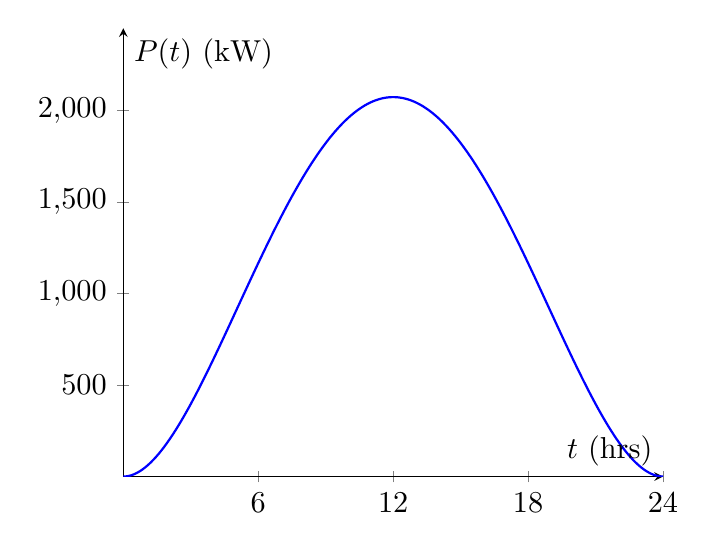
\begin{tikzpicture}
		\begin{axis}
		[axis lines = center, xmin = 0, xmax = 24, xlabel = $t$ (hrs),
		ymin = 0, ymax = 2450, ylabel = $P(t)$ (kW),
            xtick={6, 12, 18, 24}]
		\addplot[blue, thick, samples=200, domain =0:24] {0.1*x^2*(x-24)^2};
		\end{axis}
	\end{tikzpicture}
	\caption{Power consumption of a household in a day}
	\label{fig:power}
\end{figure}

To determine the total energy use, we need to evaluate $\int_{0}^{24} 
\frac{1}{10}t^2(t-24)^2\,dt$. First, we expand the polynomial:\\
$$E_{tot} = \frac{1}{10} \int_{0}^{24} t^2 (t^2-48t+576)\,dt = 
\frac{1}{10}\int_{0}^{24} t^4 - 48t^3 + 576t^2\,dt$$
$$= \frac{1}{10}\int_{0}^{24} t^4\,dt - \frac{24}{5}\int_{0}^{24} 
t^3\,dt + \frac{288}{5}\int_{0}^{24} t^2\,dt$$\\
Using the Power Rule to determine the antiderivatives of $t^4$, $t^3$, 
and $t^2$, we see:\\
$$=\frac{1}{10}[\frac{1}{5}t^5]|_{0}^{24} - \frac{24}{5}
[\frac{1}{4}t^4]|_{0}^{24} + \frac{288}{5}[\frac{1}{3}t^3]|_{0}^{24} 
= 26542.1 Whr = 26.5421 kWhr$$

\subsection{Definite Integrals Practice}
\begin{Exercise}[label=FTC2]
	Evaluate the following integrals:
	\begin{enumerate}
	\item $\int_1^4 t^{-3/2}\,dt$
	\end{enumerate}
\end{Exercise}

\begin{Answer}[ref=FTC2]
	\begin{enumerate}
	\item The antiderivative of $t^{-3/2}$ is $\frac{-2}{\sqrt{t}}$. 
	Therefore, the integral is equal to $[\frac{-2}{\sqrt{t}}]_1^4 = 
	\frac{-2}{\sqrt{4}} - \frac{-2}{\sqrt{1}} = -1 + 2 = 1$. 
	\end{enumerate}
\end{Answer}

\begin{Exercise}[label=FTC3]
	[This question was originally presented as a multiple-choice, 
	no-calculator problem on the 2p Calculus BC exam.] The graph of a 
	differentiable function $f$ is shown in the graph. $h(x) = \int_0^x 
	f(t)\,dt$. Rank the relative values of $h(6)$, $h'(6)$, and $h''(6)$ 
	from lowest to highest.
	
	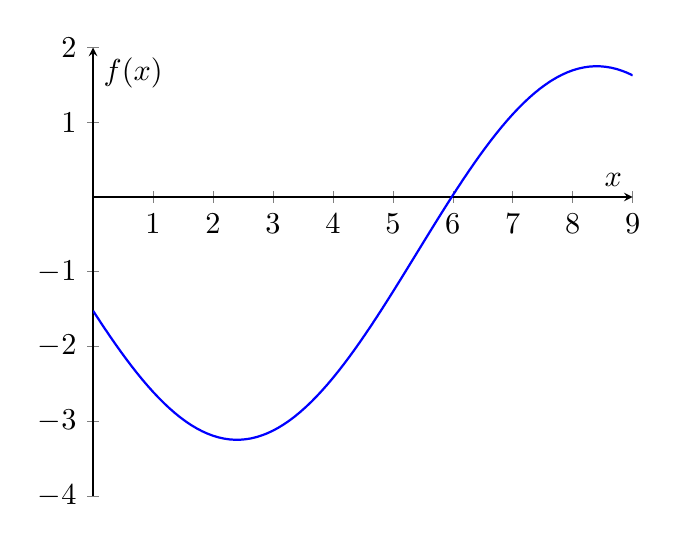
\begin{tikzpicture}
		\begin{axis}
		[axis lines = center, xlabel = $x$, ylabel = $f(x)$,
		xmin = 0, xmax = 9, xtick = {1, 2, 3, 4, 5, 6, 7, 8, 9},
		ymin = -4, ymax = 2, ytick = {-4, -3, -2, -1, 1, 2}]
		\addplot[blue, thick, samples=100, domain = 0:9]
		{2.5*sin(30*(x+6.6))-0.75};
		\end{axis}
	\end{tikzpicture}
\end{Exercise}

\begin{Answer}[ref=FTC3]
According to FTC, $h'(x) = f(x)$ and $h''(x) = f'(x)$. Examining the 
graph, we see that the curve lies below the $x$-axis for $0<x<6$, 
which means that $h(6) = \int_0^6 f(t)\,dt < 0$. $h'(6) = f(6) = 0$ 
and $h''(6) = f'(6) > 0$. Therefore, $h(6) < h'(6) < h''(6)$. 
\end{Answer}

\begin{Exercise}[label=defint6]
	The graph of $f'$ is shown in the graph and consists of a semi-circle 
	and two line segments. If $f(2) = 1$, then what is $f(-5)$?\\
	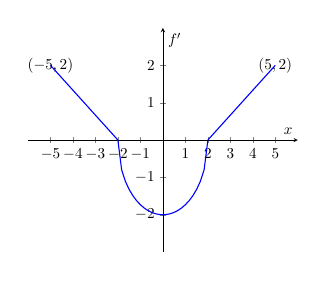
\begin{tikzpicture}[scale = 0.5]
		\begin{axis}
		[axis lines = center, xmin = -6, xmax = 6, xlabel = $x$,
		xtick = {-5, -4, -3, -2, -1, 1, 2, 3, 4, 5},
		ymin = -3, ymax = 3, ylabel = $f'$, ytick = {-2, -1, 2, 1}]
		\addplot[blue, thick]coordinates{(-5, 2) (-2, 0)};
		\node[] at (5, 2) {$(5, 2)$};
		\node[] at (-5, 2) {$(-5, 2)$};
		\addplot[blue, thick]coordinates{(5, 2) (2, 0)};
		\addplot[blue, thick, domain = -2:2]{- sqrt(4 - x^2)};
		\end{axis}
	\end{tikzpicture}
\end{Exercise}

\begin{Answer}[ref=defint6]
	We know that $f(2) = \int_{-5}^2 f'(x)\,dx + f(-5)$. Examining the 
	graph, we know that $\int_{-5}^2 f'(x)\,dx = frac{1}{2}(3)(2) - 
	\frac{1}{2}\pi(2^2)$ (the area of the triangle above the $x$-axis 
	less the area of the semi-circle below the axis). Therefore, $f(-5) 
	= f(2) - \int_{-5}^2 f'(x)\,dx = 1-(3-2\pi) = 2\pi-2$
\end{Answer}




\graphicspath{{../../Chapters/gas/en_US}}
\chapter{The Physics of Gases}


Now,  let's say you start to heat the helium inside the balloon.  As the temperature goes up,  the molecules inside will start to move faster.

Remember that the kinetic energy of an object with mass $m$ and velocity $v$ is given by

$$k = \frac{1}{2} m v^2$$

So, you could say "As the temperature of the gas increases,  the kinetic energy of the molecules increases."   But a physicist would say "The temperature of the gas is how we measure its kinetic energy."

\subsection{A Statistical Look At Temperature}

If you say "This jar of argon gas is 25 degrees Celsius,"  you have told me about the \emph{average} kinetic energy of the molecules in the jar.  
However,  some molecules are moving very slowly.  Others are moving really,  really fast. 

We could plot the probability distribution of the speeds of the molecules.  For argon at 25 degrees Celsius,  it would look like this:

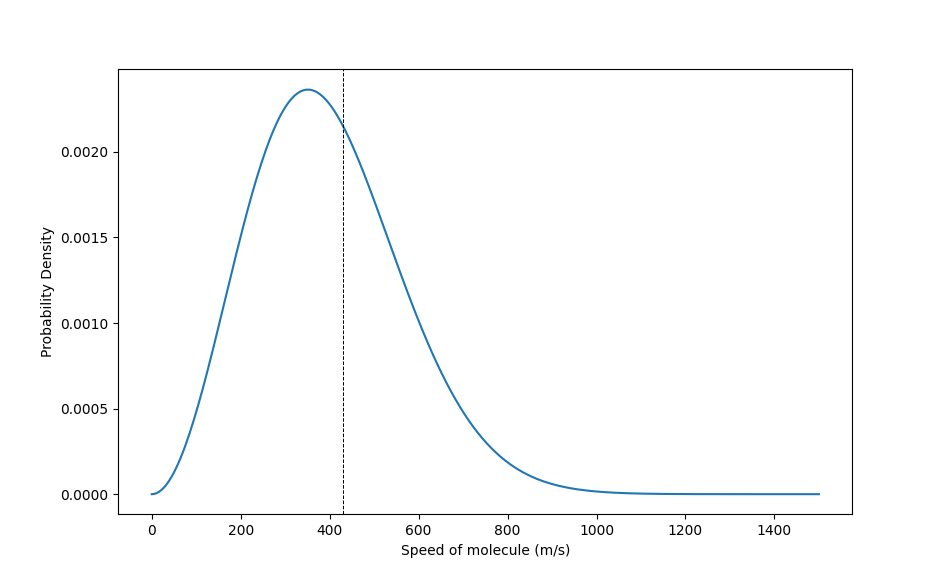
\includegraphics[width=\textwidth]{ar_plot.png}

The temperature,  remember,  is determined by the average kinetic energy of the molecules.  Some molecules are moving slowly and have less kinetic energy than the average.  Some molecules are moving very quickly and have more kinetic energy.  The dotted line is the divider between the two groups: molecules moving at speeds to the left of the line have less kinetic energy than average; those on the right have more kinetic energy than average.

Where is that line?  That is the RMS of the speeds of the molecules.  That is, if we measured all the speeds of all the molecules  $s_1, s_2, s_3, \ldots, s_n$, that line would be given by the root of the mean of the squares:

$$v_{rms} = \sqrt{\frac{1}{n} \left( s_1^2 + s_2^2 + s_3^2 + \ldots s_n^2 \right)}$$

If you have the same gas at a lower temperature, the distribution shifts toward zero:

Here is probability distribution of molecular speeds for argon gas at 25 degrees and -100 degrees Celsius.

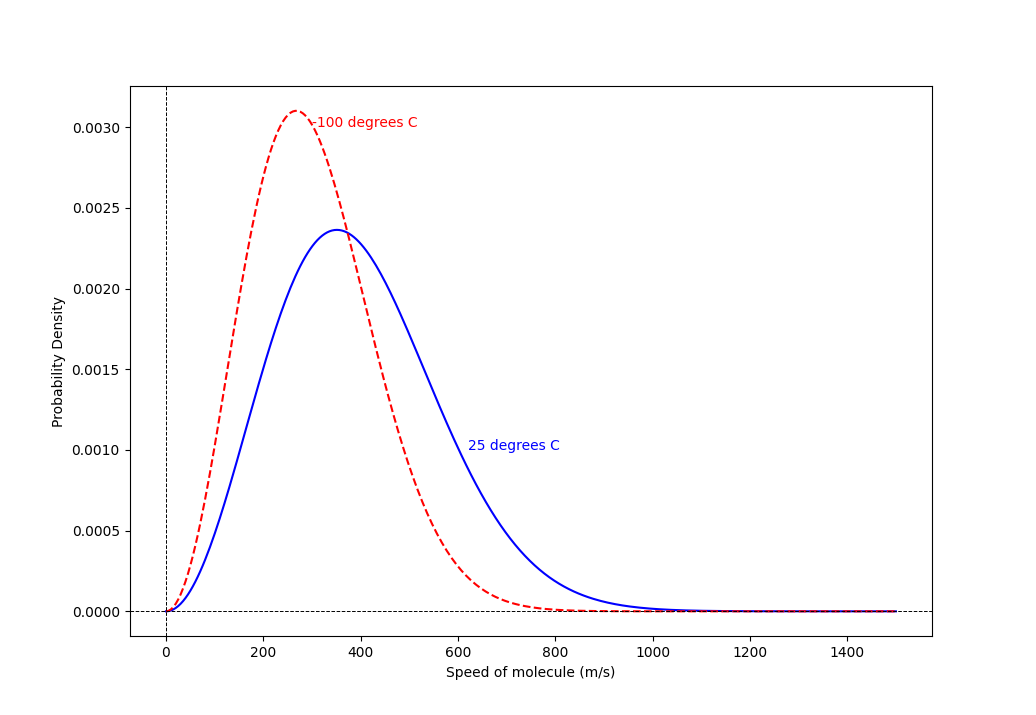
\includegraphics[width=\textwidth]{ar2_plot.png}

\subsection{Absolute Zero and Degrees Kelvin}

If you keep lowering the temperature,  eventually all the molecules stop moving.  This is known as \newterm{absolute zero} -- you
 can't make anything colder than absolute zero.   Absolute zero is -273.15 degrees Celsius.
 
Besides Celsius and Fahrenheit, there is a third temperature system: Kelvin.  The Kelvin has the same scale as Celsius, but it starts at absolute zero.   
So,  0 degrees Celsius is 273.15 degrees Kelvin.    And 100 degrees Celsius is 373.15 degrees Kelvin.

Any time you are working with the physics of temperature, you will use Kelvin.

Sometimes, when reading about gases, you will see "STP"  which stands for "Standard Temperature and Pressure."  STP is defined to be $0^\circ$ Celsius and 100 kPa.

\section{Temperature and Volume}

Let's say you have a half-full air mattress in a field with a person lying on it around dawn.   The weight of the person will keep the pressure of the air inside constant (or pretty close).  

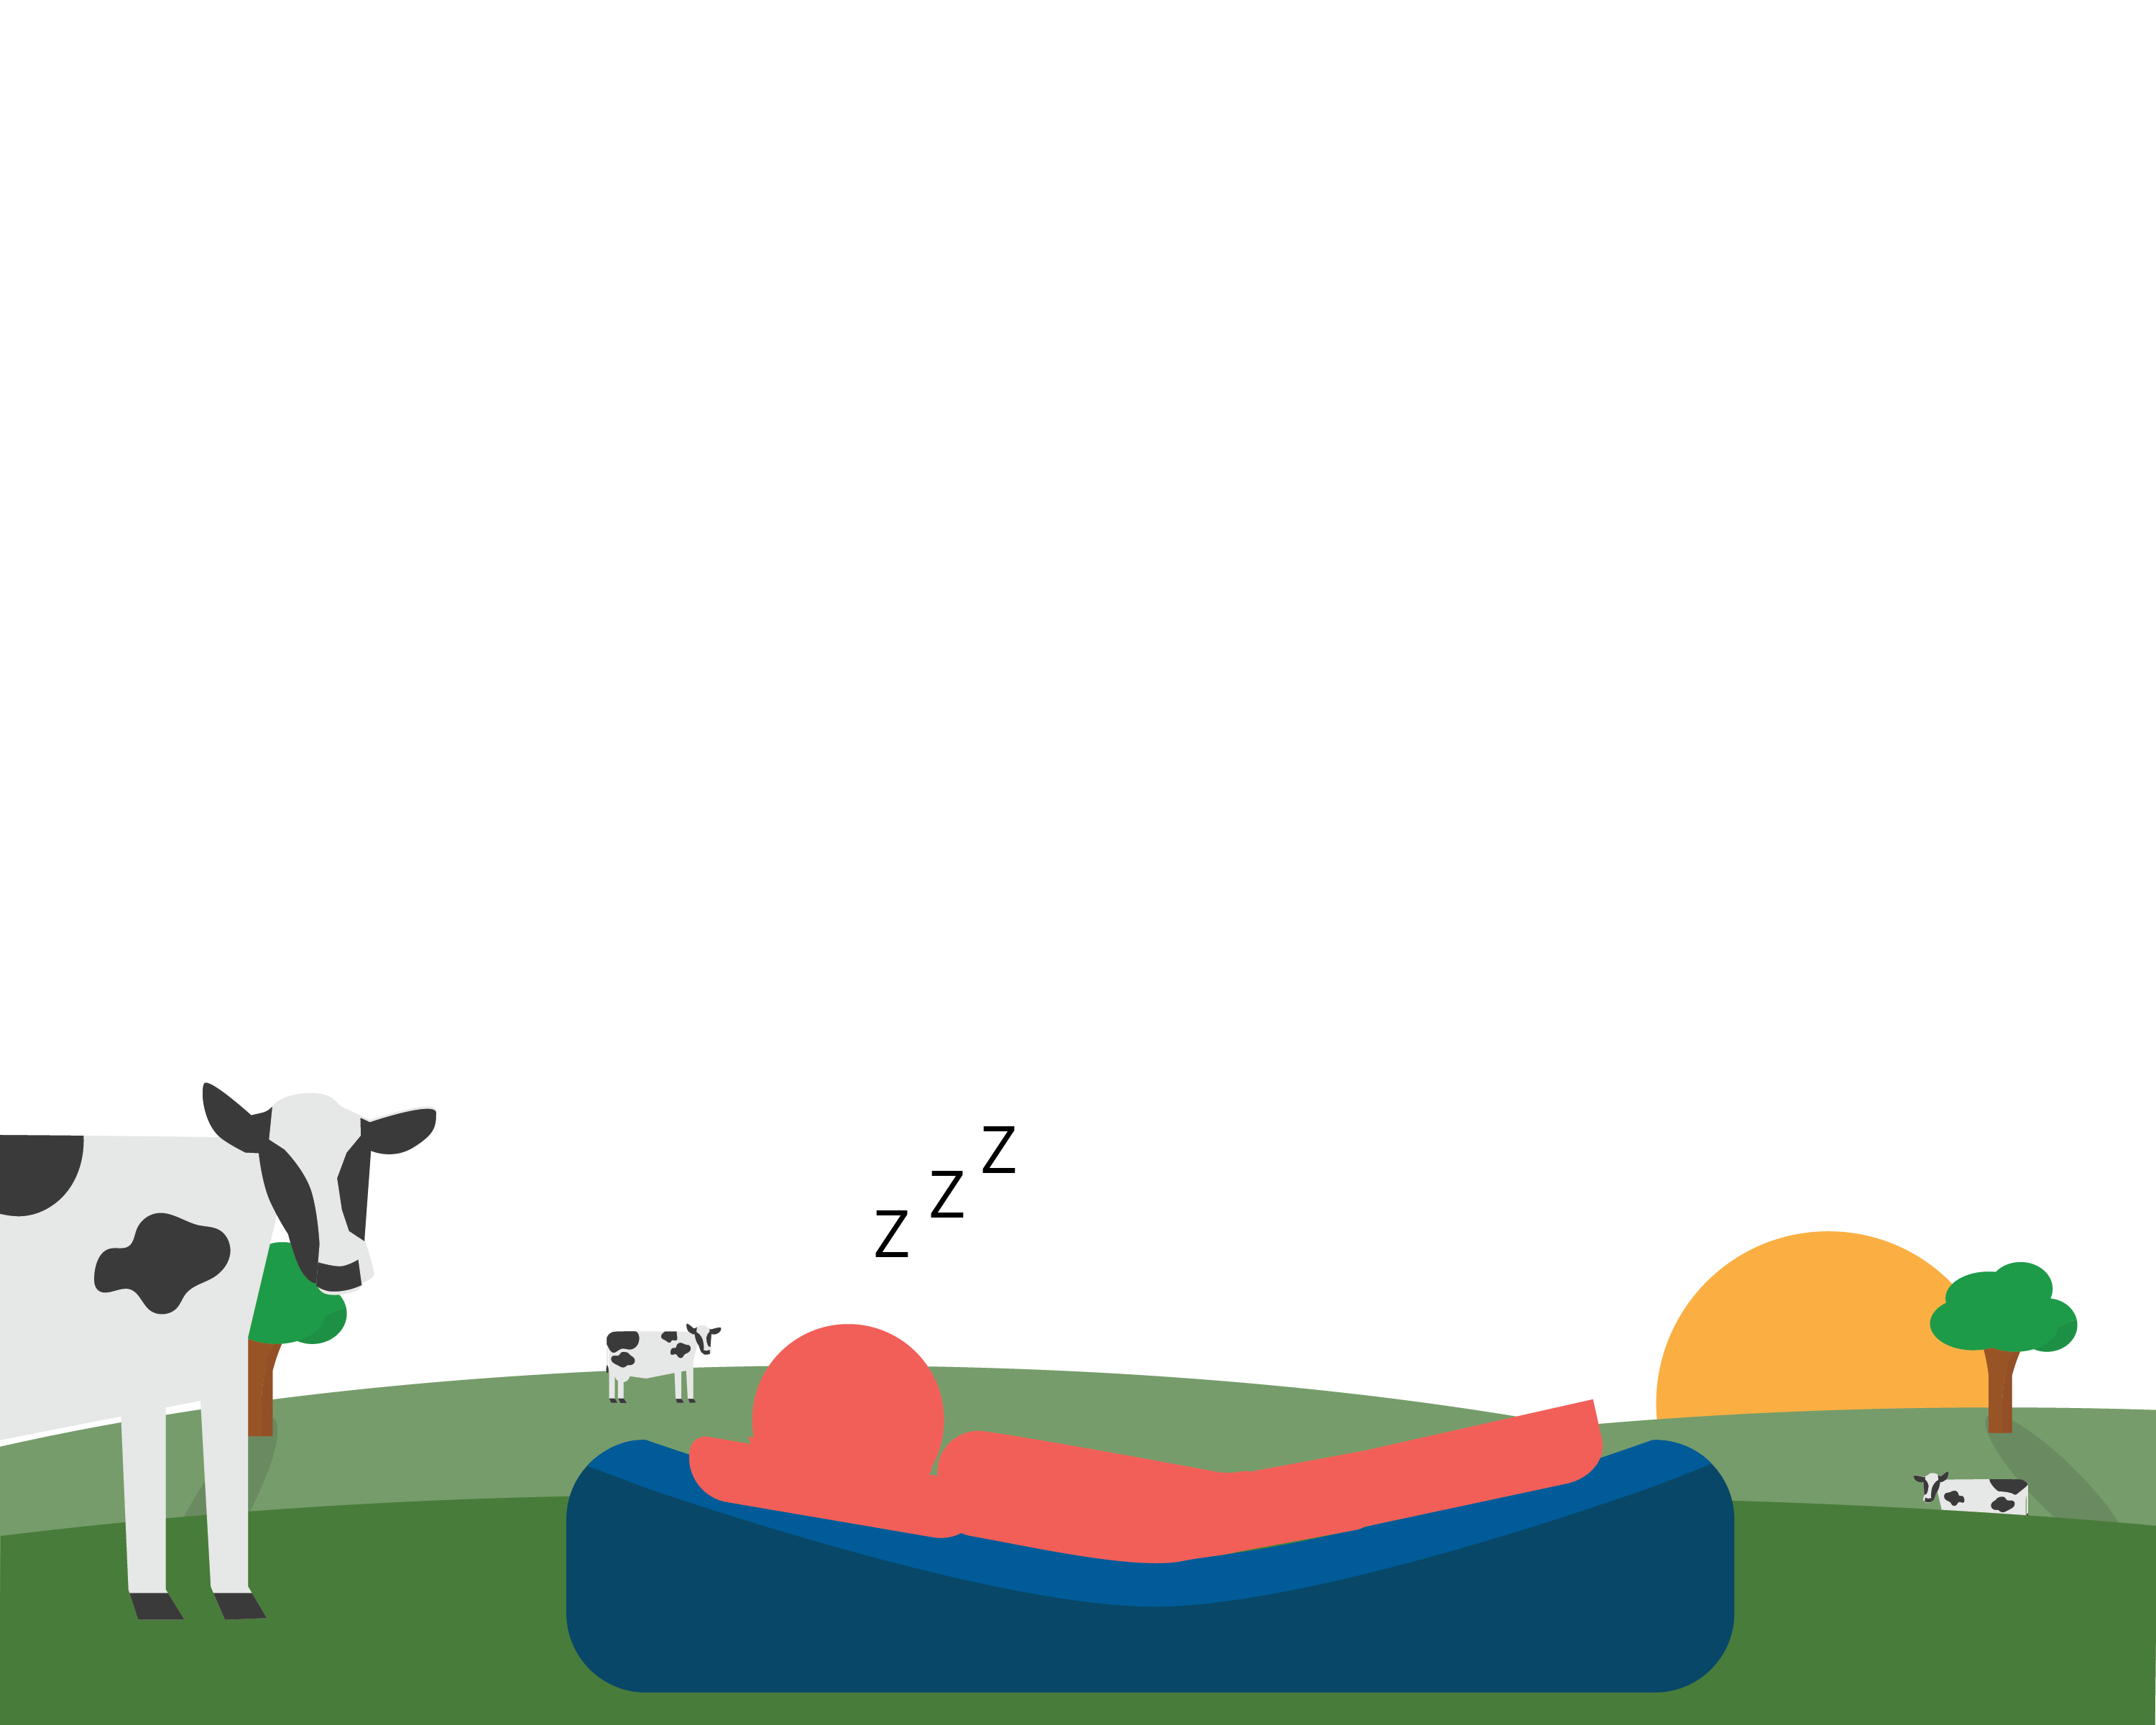
\includegraphics[width=\textwidth]{airMattress1.png}


The molecules in the mattress are not entering or leaving that mattress.  However, as the sun rises,  the air inside will get warmer and expand.  The person will be gently lifted by the expanding air.  You might wonder: how much will the air expand?

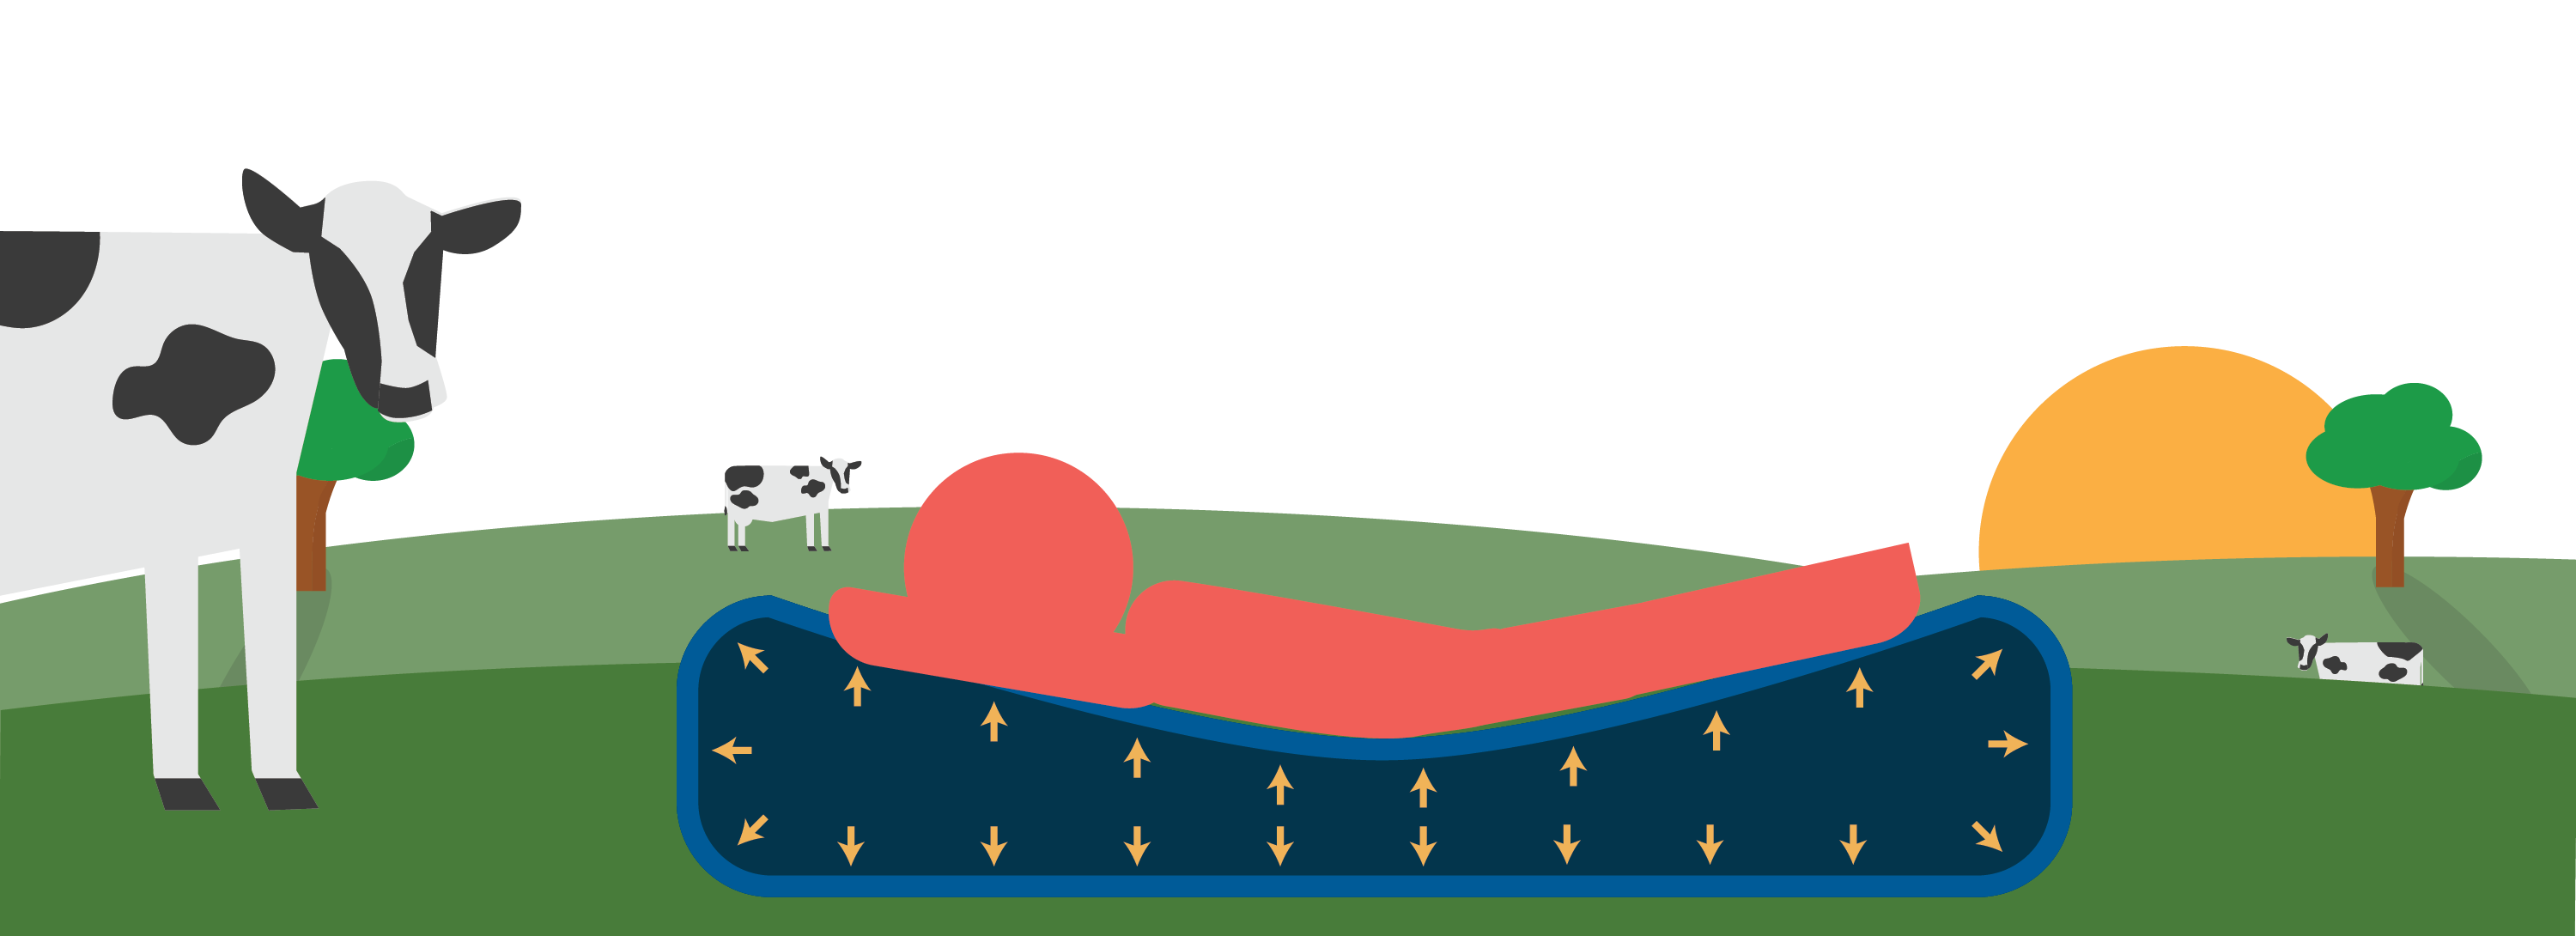
\includegraphics[width=\textwidth]{airMattress2.png}
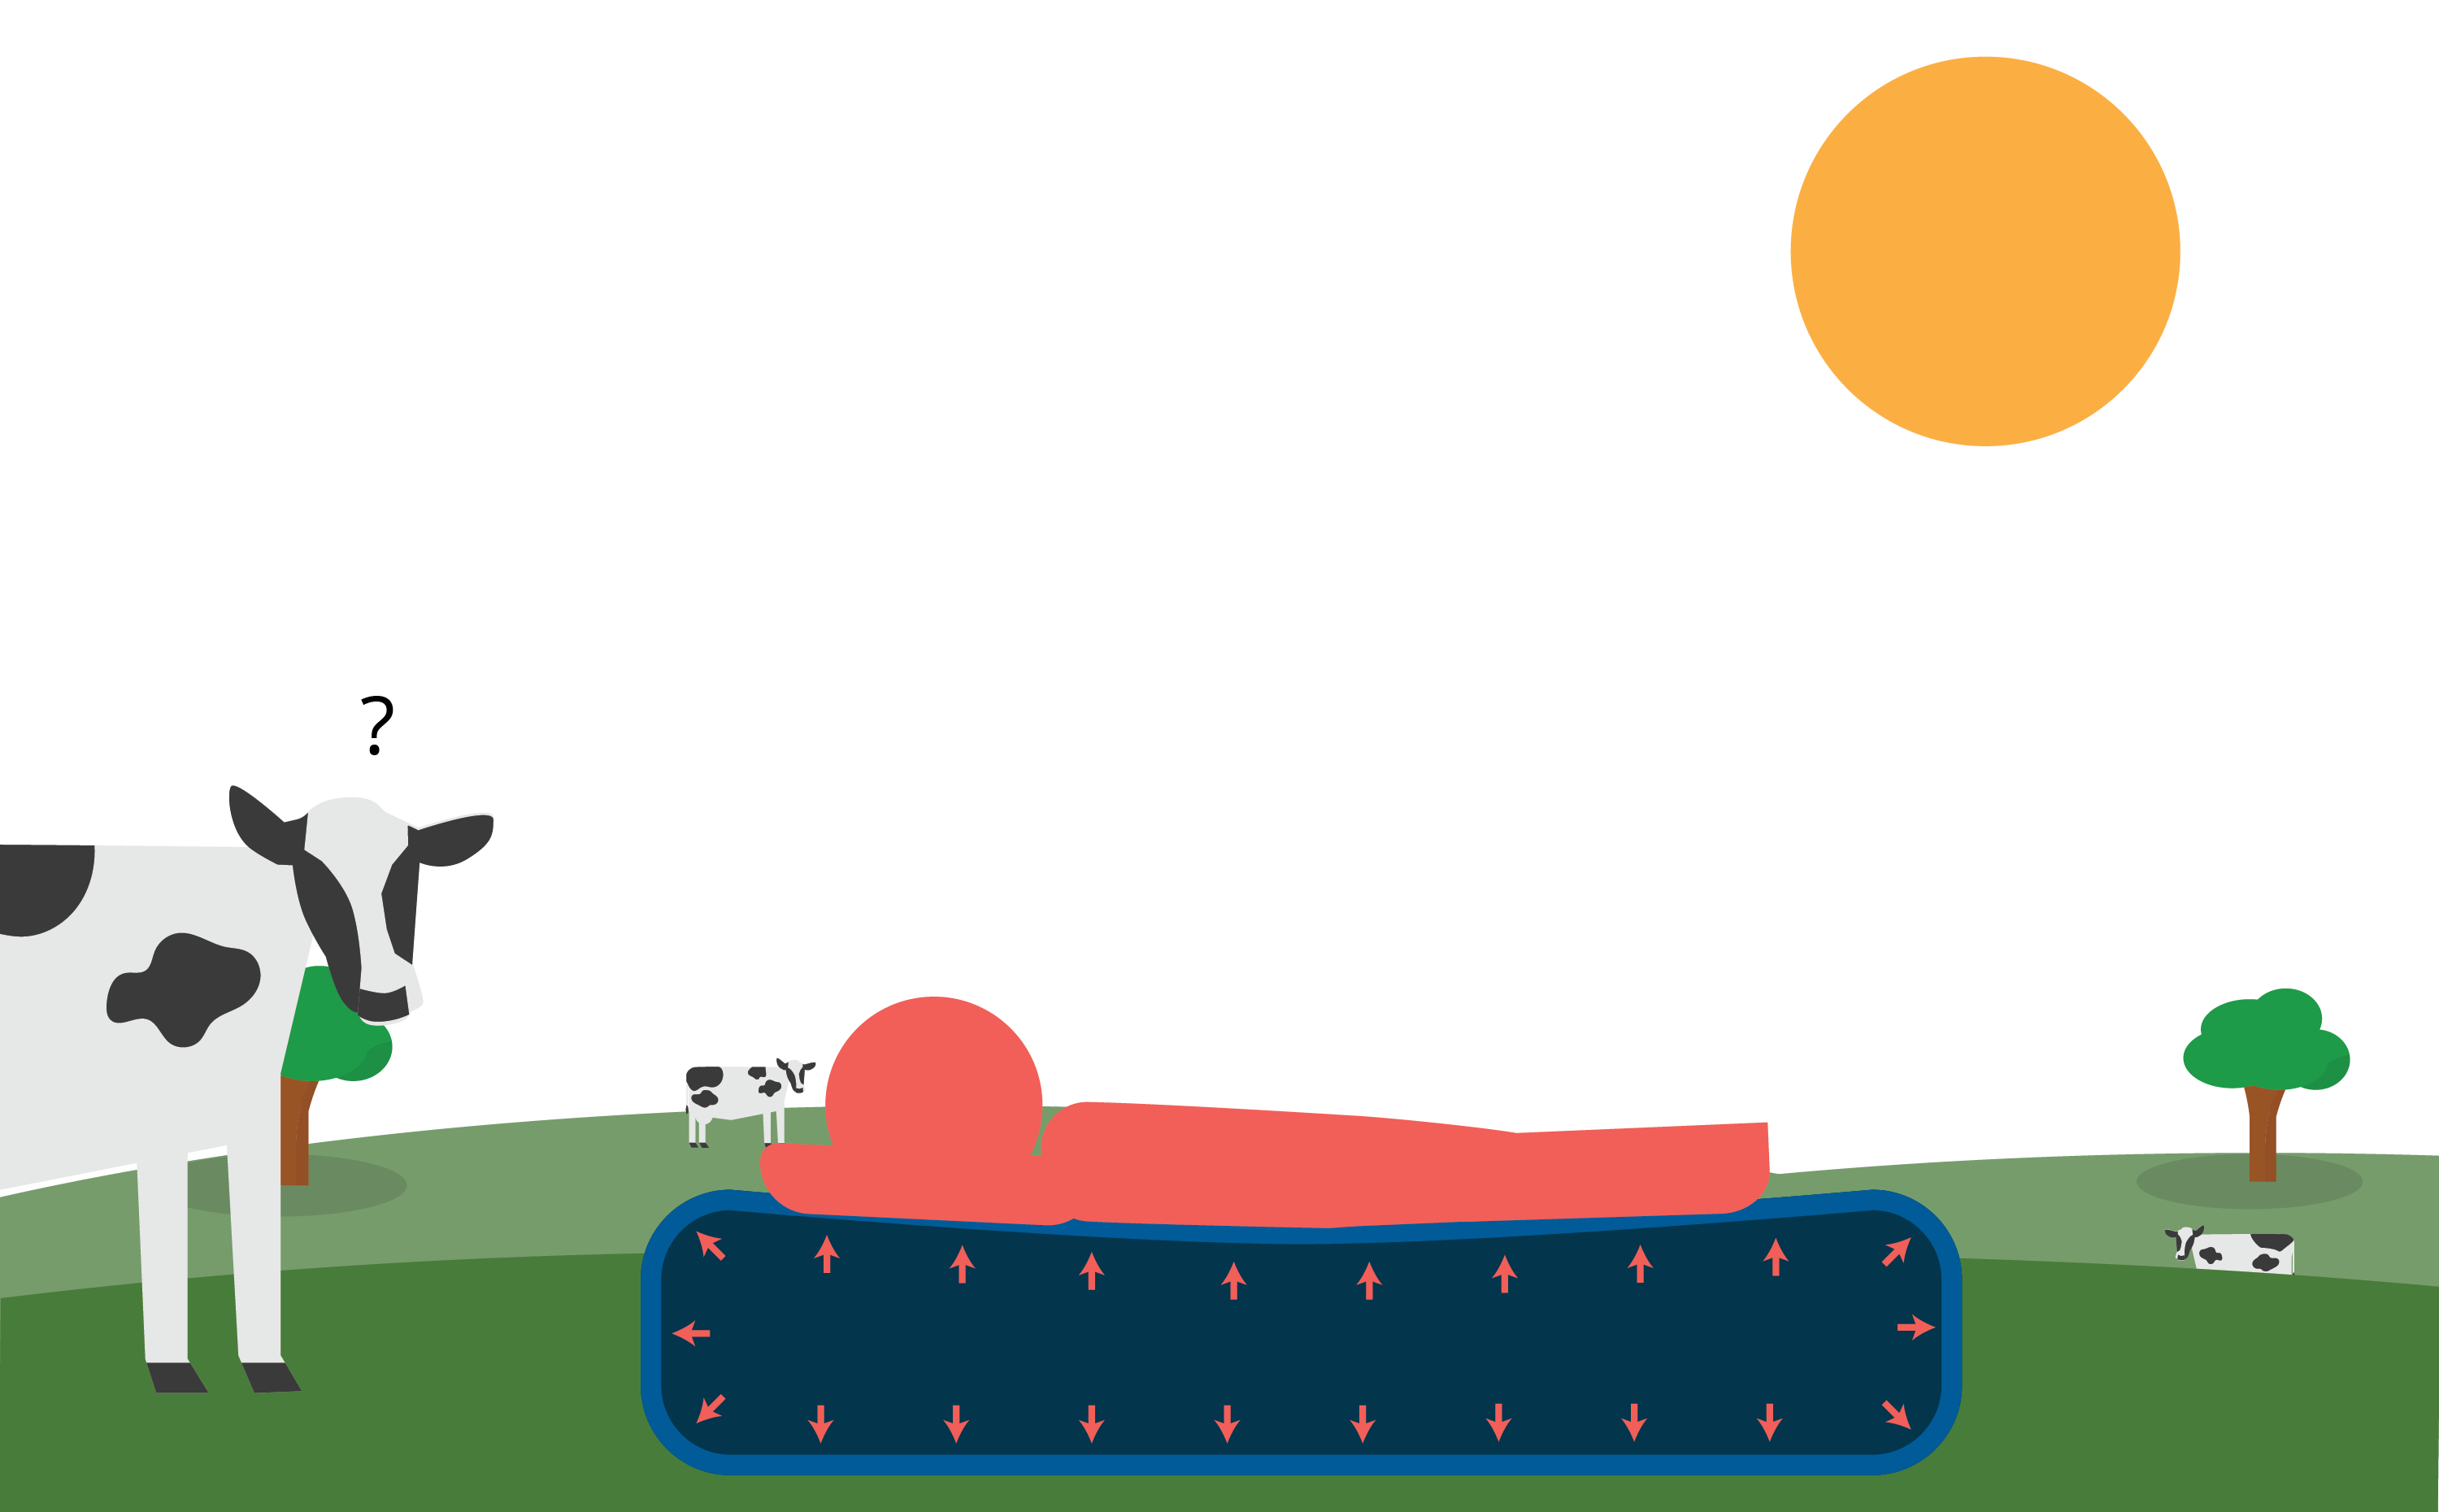
\includegraphics[width=\textwidth]{airMattress3.png}


If you have constant pressure and and a constant number of molecules,  the volume of the gas is proportional to the temperature in Kelvin:

$$V \propto T$$

\begin{Exercise}[title={Temperature and Volume},  label=temp_vol]
  
At dawn, the air inside mattress at dawn has a volume of 1000 liters and a temperature of 12 degrees Celsius.

At noon,  that same air has a temperature of 28 degrees Celsius.  The pressure on the gas has not changed at all.

What is the volume of the gas at noon?

\end{Exercise}
\begin{Answer}[ref=temp_vol]

First, we convert the temperatures into Kelvin:  
\begin{itemize}
\item Dawn: $12 + 273.15 = 285.15$
\item Noon: $28 + 273.15 = 301.15$
\end{itemize}

So, the temperature $T$ has increased by a factor of $\frac{301.15}{285.15} \approx 1.056$

Thus the volume of the air mattress has also increased by a factor of 1.056.  

So the air mattress that had a volume of 1000 liters at dawn,  will have a volume 1056 liters at noon.

\end{Answer}

Note: Volume and temperature are only proportional as long as the substance is a gas.   We will talk about liquids and solids soon.

\section{Pressure and Volume}

As you increase the pressure on a gas,  the molecules will get pushed closer together,  and the volume will decrease.

For example,  if you put the cap on an empty plastic bottle and squeeze it.   As you put the gas inside the bottle under pressure,  its volume will decrease. 

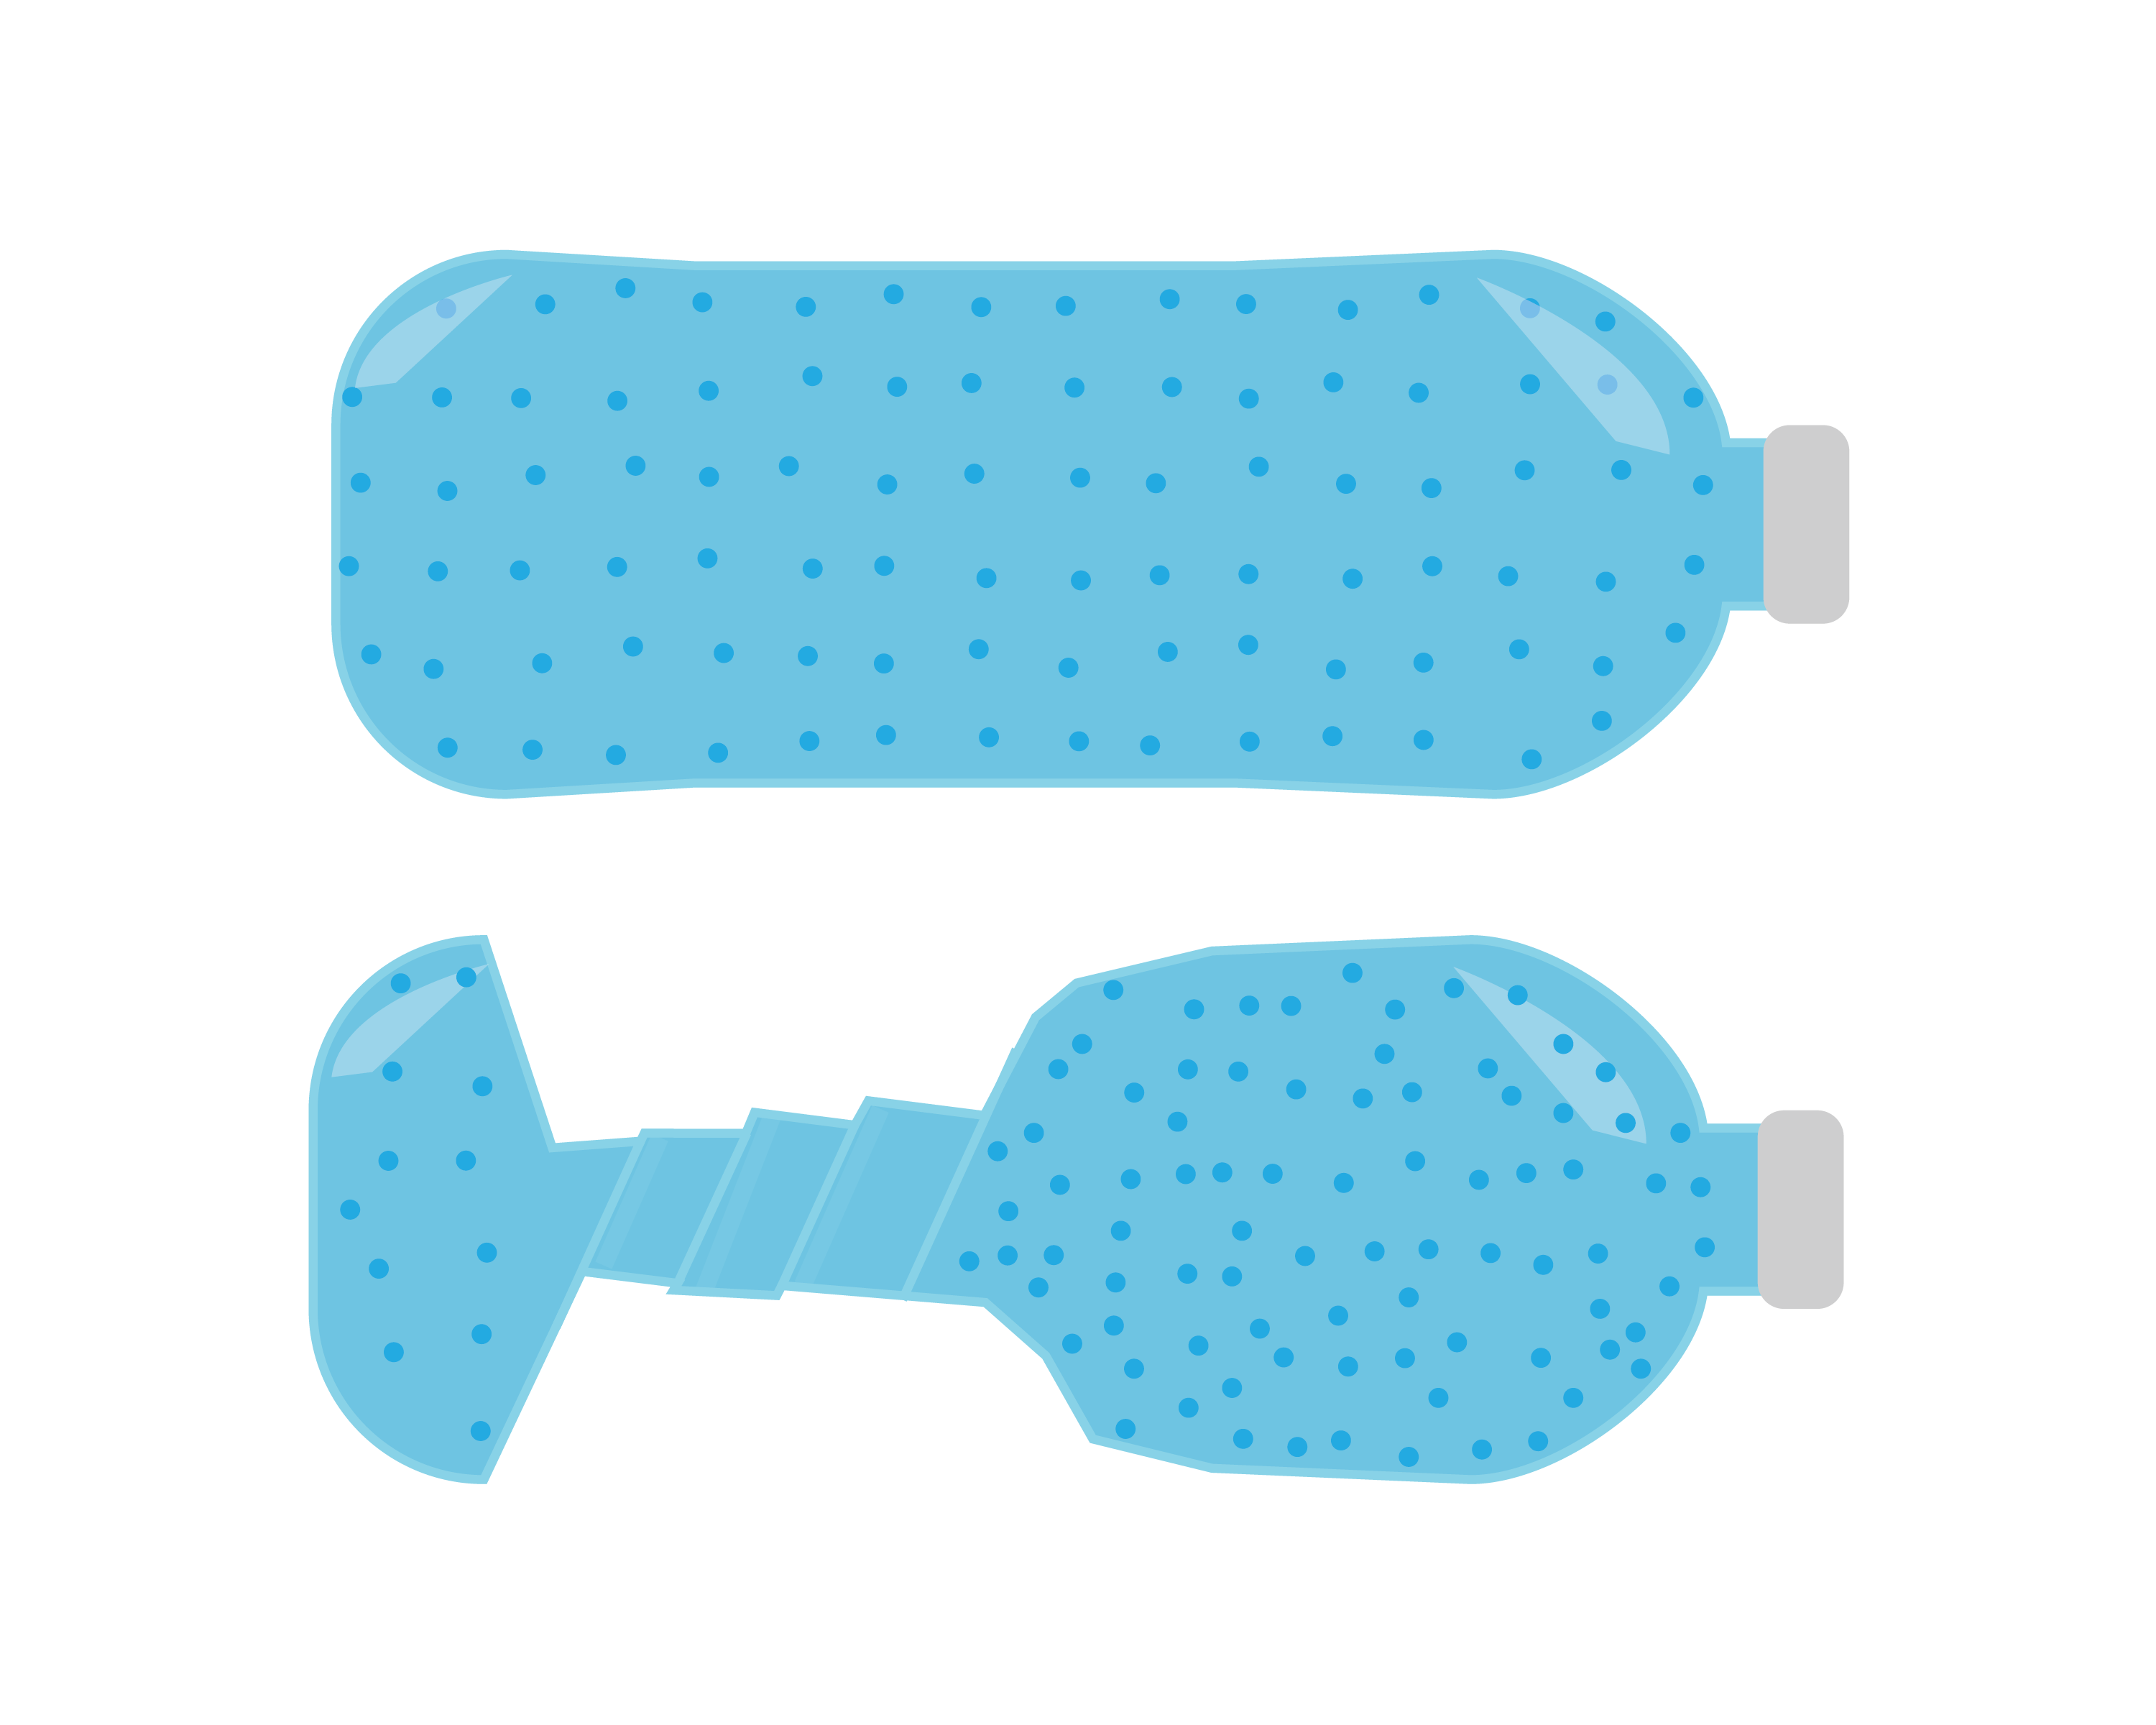
\includegraphics[width=0.75\textwidth]{waterBottle.png}


If you keep the number of molecules and the temperature constant,  the pressure of the gas and its volume are inversely proportional:

$$P \propto \frac{1}{V}$$

"But," you say with disbelief, "if I increase the pressure on my empty water bottle from 5 kPa to 10 kPa,  the volume inside won't decrease by half!"

Don't forget that the air inside the bottle is under 101 kPa of atmospheric pressure before you even start to squeeze it.

\begin{Exercise}[title={Temperature and Volume},  label=temp_vol]
  
At an altitude where the atmospheric pressure is 100 kPa,  you seal air in a 1 liter water bottle.

Squeezing the water bottle,  you raise the internal pressure by 20 kPa  What is the volume inside the bottle now?

\end{Exercise}
\begin{Answer}[ref=temp_vol]

What is the pressure in kPA?  
\begin{itemize}
\item Before squeezing: 100 kPa
\item While squeezing: 120 kPa
\end{itemize}

So, the pressure $P$ has increased by a factor of $\frac{120}{100} = 1.2$

$1/1.2 \approx 0.833$

The air in the bottle had a volume of 1 liter before squeezing, so it has a volume of 833 milliliters while being squeezed.

\end{Answer}

\section{The Ideal Gas Law}

You are gradually getting an intuition for the relationship between the number of molecules, the volume, the pressure, and the temperature of a gas.
We can actually bring these together in one handy equation.

\begin{mdframed}[style=important, frametitle={Ideal Gas Law}]

$$PV = nRT$$

where:
\begin{itemize}
\item $P$ is the pressure in pascals
\item $V$ is the volume in cubic meters
\item $n$ is the number of molecules in moles
\item $R$ is the molar gas constant: 8.31446
\item $T$ is the temperature in Kelvin
\end{itemize}

(You can remember this as the "Pivnert.")

\end{mdframed}

From the name,  you might predict the following: The Idea Gas Law is not 100\% accurate.   But for most purposes,  it works remarkably well.  

Notice that the ideal gas law says nothing about what kind of gas it is; it works regardless.

\begin{Exercise}[title={Ideal Gas Law},  label=ideal_gas]
  
You have a cylinder containing $O_2$.  The chamber inside has a radius of 12 cm and a length of 50 cm.  
The temperature inside the cylinder is 20 degrees Celsius.
The pressure inside the tank is 600 kPa.

How many moles of $O_2$ are inside?

\end{Exercise}
\begin{Answer}[ref=ideal_gas]

First, let's convert the known values to the right unit:
\begin{itemize}
\item Radius = 0.12 m
\item Length = 0.5 m
\item $T = 20 + 273.15 = 293.15$ degrees Kelvin
\item $P = 600 \text{ kPa } = 600,000 \text{ Pa }$
\end{itemize}

The volume of the cylindrical chamber is $V = \pi r^2 h = \pi (0.12)^2 0 (0.5) \approx 0.0226$.

The Ideal Gas Law tell us that $PV = nRT$.  We are solving for $n$.

$$n = \frac{PV}{RT} = \frac{(600,000)(0.0226)}{(8.31446)(293.15)} \approx 5.68 \text{ moles of } O_2$$

\end{Answer}

\section{Molecules Like To Stay Close to Each Other}

When two molecules get close to each other a few things can happen:
\begin{itemize}  
\item They can under go a chemical reaction: electrons are exchanged or shared and a different molecule or molecules come into existence.  
This is the realm of chemistry, and we won't go into it in this course.
\item One or both of them have so much kinetic energy that they just pass each other or bounce off each other.  This is what happens in a gas.
\item The two molecules can "stick" together.  This is what happens in a liquid or a solid.
\end{itemize}

Why do they stick together if they aren't combined in a chemical reaction?

First, they don't get \emph{too close}.  If they get too close,  their electron clouds repel each other with a strong force.  
This is what happens in a gas when two molecules bounce off of each other.

But if the molecules are quite close to each other,  there are forces that will attract them toward each other.  
These intermoleculare forces are beyond the scope of this course, but they called Van der Waals forces and hydrogen bonds.   
The strength of these forces vary based on the two molecules involved. 

Which is why some of the matter around you is in gas form (molecules that don't stick together at the temperature and pressure you are living in because they have weak attractive forces) and some is non-gas 
(gangs of molecules with stronger attraction that makes them clump together as a liquid or a solid at that same temperature and pressure).

But.  What if we change the temperature and pressure,  we can change if and how the molecules clump together.  
This is known a \newterm{phase change}; We will cover it soon.
\graphicspath{{../../Chapters/temp_kinetic/en_US}}
\chapter{Kinetic Energy and Temperature of a Gas}

As mentioned in the previous chapter,   for a particular gas,  the temperature (in Kelvin) is proportional to the average kinetic energy of the individual molecules. 

Perhaps you want to warm 3 moles of helium gas (trapped in a metal cylinder) from 10 degrees Celsius to 30 degrees Celsius.   
How would you compute exactly how many Joules of energy this would require?

The amount of energy necessary to raise one mole of a molecule by one degree is known as \newterm{molar heat capacity}.  
(The molar heat capacity of liquid water, for example, is 75.38 J per mole-degree.)

With gases, are actually two different possible situations:
\begin{enumerate}
\item Constant volume: As you heat the gas,  the pressure and the temperature increase.  This molar heat capacity is usually denoted as $C_{V,m}$.
\item Constant pressure: As you heat the gas,  the temperature and the volume increase.  This molar heat capacity  is usually denoted as $C_{P, m}$.
\end{enumerate}

All gases made up of one atom (Helium, for example, is a monoatomic gas.) have the same values for $C_{V,m}$ and $C_{P,m}$:

$$C_{V,m} = \frac{3}{2}R \approx 12.47 \text{ Joules per mole-degree}$$

$$C_{P,m} = \frac{5}{2}R \approx 20.8  \text{ Joules per mole-degree}$$

(Remember from last chapter that $R$ is the ideal gas constant $\approx 8.31446$ Joules per mole-degree.)

\begin{Exercise}[title={Warming Helium},  label=warming_helium]

You have 3 moles of helium.  
  
\begin{enumerate}

\item How many Joules would be required to warm 3 moles of helium gas by 20 degrees Celsius at constant volume?  

\item How many Joules would be required to warm 3 moles of helium gas by 20 degrees Celsius at constant pressure?  

\end{enumerate}


\end{Exercise}
\begin{Answer}[ref=warming_helium]

$E = C_{V,m} (3 \text{ moles }) (20 { degrees Celsius }) = (12.47)(3)(20) = 748 \text{ Joules }$

$E = C_{V,m} (3 \text{ moles }) (20 { degrees Celsius }) = (20.8)(3)(20) = 1247 \text{ Joules }$
\end{Answer}

\section{Molecule Shape and Molar Heat Capacity}

We told you that gases made up of one atom have the same values for $C_{V,m}$ and $C_{P,m}$:

$C_{V,m} = \frac{3}{2}R \approx 12.47 \text{ Joules per mole-degree}$

$C_{P,m} = \frac{5}{2}R \approx 20.8  \text{ Joules per mole-degree}$

For any molecule, it is generally true that 

$$C_{P,m} \approx C_{V,m} + R$$

It is also true that for any molecule,  there is some integer $d$ such that

$$C_{V, m} \approx \frac{d}{2}R$$

For example, for all monoatomic gases,  $d = 3$.  For diatomic gases (like $N_2$ and $O_2$,  $d$ is 5.

$d$ is known as the \newterm{degree of freedom} of the molecule.  When you study chemistry, they will teach you to predict $d$ based on the shape of the molecule. 

Here are the relevant numbers for some gases you are likely to work with:

\begin{tabular}{r|c|c| c| c}
Gas & type & $C_{V,m}$ & $C_{P,m}$ & $d$\\
\hline
$He$ &  monoatomic & 12.4717 & 20.7862 & 3 \\
$Ar$ & monoatomic & 12.4717 & 20.7862 & 3 \\
$O_2$ & diatomic & 21.0 & 29.38 & 5\\
$N_2$ & diatomic & 20.8 & 29.12 & 5\\
$HO_2$ (water vapor) & 3 atoms &  28.03 & 37.47 & 7 \\
$CO_2$ & 3 atoms & 28.46 & 36.94 & 7\\
\end{tabular}

\section{Kinetic Energy and Temperature}

For a sample of a gas, we can calculate its kinetic energy based on its molar heat capacity,  the number of molecules, and the temperature:

$$E_K = C_{V,m} n T$$

where

\begin{itemize}
\item $E_K$ is the kinetic energy in Joules
\item $C_{V,m}$ is the molar heat capacity of the gas at constant volume
\item $n$ is the number of molecules in moles
\item $T$ is the temperature in Kelvin
\end{itemize}


\begin{Exercise}[title={Warming Helium Revisited},  label=warming_helium2]

How much kinetic energy does 3 moles of helium have at 10 degrees Celsius?

How much kinetic energy does 3 moles of helium have at 30 degrees Celsius?

What is the difference?

\end{Exercise}
\begin{Answer}[ref=warming_helium2]

10 degrees Celsius is 283.15 degrees Kelvin.  30 degrees Celsius is 303.15.

For any gas:

$$E_K =C_{V,m} n T$$

And $C_{V,m} = 12.47$ for all monoatomic gases.

So the energy at 10 degrees Celsius:

$$E_1 = (12.47)(3)(283.15) = 10,594 \text{ Joules}$$

The energy at 30 degrees Celsius:

$$E_2 = (12. 47)(3)(303.15) = 11,342 \text{ Joules}$$

The difference?

$$E_2 - E_1 = 11,342 - 10,594   = 748 \text{ Joules }$$

Which is consistent with your earlier exercise.

\end{Answer}

\section{Why is $C_{V,m}$ different from $C_{P,m}$?}

What if, instead of keeping the volume constant while we heat the molecules in the helium tank,  we keep the pressure constant and let the gas expand?  
The change in kinetic energy is the same: 748 Joules.

However,  we know that the molar heat capacity if we keep pressure constant is $\frac{5}{2}R$,  so  heating will require $\frac{5}{2}R(3)(20) = 1247$ Joules.  

What happened to the 499 missing Joules!?  Thermodynamics tells us energy is neither created nor destroyed.  So it must have gone somewhere.

That energy was used pushing against the pressure as the gas expanded.  For example,  maybe the sample was in a balloon in space -- the extra energy stretched the surface of the balloon.  

The 499 Joules were converted into potential energy.   

\section{Work of Creating Volume Against Constant Pressure}

Let's imagine that you had a total vacuum (zero pressure) with a piston.  As you pulled the piston out,  you would be pulling against  the atmospheric pressure.  How much energy would that require?

If you increased the volume of the vacuum by $V$ against a pressure of $P$,   you would do $VP$ work.

Let's check to make sure the 499 Joules mentioned above makes sense with this in mind.

No initial pressure was given in the problem, so let's just make one up and see how things work out: 100 kPa.  Using the ideal gas law,  the initial volume would be:

$$V_1 = \frac{n R T}{P} = \frac{(3)(8.31446)(283.15)}{100,000} = 0.07063\text{ cubic meters}$$

The volume after we heated the gas and let it expand against 100 kPa would be:

$$V_2 = \frac{n R T}{P} = \frac{(3)(8.31446)(303.15)}{100,000} = 0.07562\text{ cubic meters}$$

So the volume increased by $0.07562 - 0.07063 = 0.00499$ cubic meters.   
Multiplying that by 100,000 pa, we get 499 Joules as we expected!

\section{Why does a gas get hotter when you compress it?}

Now imagine that there is gas inside the piston and you push on the piston to compress that air.   The work that you do is converted into kinetic energy,  and that kinetic energy raises the temperature of the gas.

So, for example,  if you had two moles of argon gas in the piston.  If you pushed the piston 0.1 meters with an average force of 50 newtons,  you will have done 5 Joules of work.

How much would 5 Joules raise the temperature of 2 mole of a monoatomic gas?  

$$\Delta T = \frac{5}{(2)(C_{V,m})} = 0.2^\circ \text{ Kelvin}$$ 

It works both ways:  compression makes a gas hotter  Decompression makes a gas colder.  You can sometimes experience the heat of compression when you pump up a bicycle tire -- as you pump the tire will get warmer.

If you compress or decompress a gas without letting any heat enter or depart,  we say the compression or decompression was \newterm{adiabatic}.  In order to solve any interesting problems about heating/cooling due to compression/decompression,  you will need to assume the process was adiabatic.

When a spacecraft enters the atmosphere,  it has to deal with a lot heat.   Some people assume that heat is due to friction of the air rubbing against the 
spacecraft at over 7,000 meters per second.  Actually,  most of the heat is due to the compression of the air as it gets pushed out of the way of the spacecraft.

\section{How much hotter?}

Let's say you have a accordion-like container filled with helium at 100 kPa (about 1 atmosphere) and 300 degrees Kelvin.  It holds 2 cubic meters.    And then you put it in a vice and quickly compress it down to 0.5 cubic meters.  Assuming it was adiabatic,  how hot would the gas inside be after the compression?

Here is the challenging part:  As you crush the container,  the temperature and the pressure in the container are both increasing.  So as you go,  it gets harder and hard to crush.  So each milliliter of volume that you eliminate requires a little more work than the milliliter before.

Let's simulate the process in python,  and then I'll give you the formula.  

In the simulation, you will start with an initial volume of 2 cubic meters and crush it down to 0.5 cubic meters in 40 steps.  At each step you will recalculate the temperature and pressure.

Then you will plot the results.  Make a file called \filename{gas\_crunch.py}:

\begin{Verbatim}
import numpy as np
import matplotlib.pyplot as plt

V_initial = 2.0 # cubic meters
V_final = 0.5 # cubic meters
step_count = 40 # steps

T_initial = 300.0 # kelvin
P_initial = 100000 # pascals

# Constants
R = 8.314462618 # ideal gas constnt
C_v =  3.0 * R / 2.0 # molar heat capacity (constant volume)

# Compute the number of moles
n = P_initial * V_initial/(R * T_initial) 
print(f"The container holds {n:.2f} moles of helium")

# How much volume do we need to eliminate in each step? 
# (in cubic meters)
step_size = (V_initial - V_final) / step_count

# For recording the state for each step
data_log = np.zeros((step_count, 3))

# Variables to update in the loop
V_current = V_initial
T_current = T_initial
P_current = P_initial

for i in range(step_count):
    # Record the current state
    data_log[i,:] = [T_current, V_current, P_current/1000.0]

    # Find how much energy to make the step at the current pressure
    E_step = step_size * P_current

    # Find how big the change in temperature will be from that energy
    delta_T = E_step / (n * C_v)

    # Update the current temperature, volume, and pressure
    T_current += delta_T
    V_current -= step_size
    P_current = n * R * T_current / V_current

print(f"Iterative:{T_current:0.3f} K, {V_current:0.3f} m3, {P_current/1000.0:0.3f} kPa")

fig, axs = plt.subplots(3,1,sharex=True, figsize=(8, 6))
axs[0].set_xlim((0,step_count))
axs[0].plot(data_log[:,0], 'k', lw=0.2)
axs[0].plot(data_log[:,0], 'r.')
axs[0].set_ylabel("Temperature (K)")

axs[1].plot(data_log[:,1],'k', lw=0.2)
axs[1].plot(data_log[:,1], 'r.')
axs[1].set_ylabel("Volume (cubic m)")

axs[2].plot(data_log[:,2], 'k', lw=0.2)
axs[2].plot(data_log[:,2], 'r.')
axs[2].set_ylabel("Pressure (kPa)")

axs[2].set_xlabel("Step")

fig.savefig('tvpplot.png')
\end{Verbatim}

When you run this,  you will see how many moles of gas there are and reasonable estimates of the temperature,  volume,  and pressure:

\begin{Verbatim}
> python3 gas_crunch.py            
The container holds 80.18 moles of helium
Iterative:733.499 K, 0.500 m3, 977.999 kPa
\end{Verbatim}

And a good plot of the intermediate values:

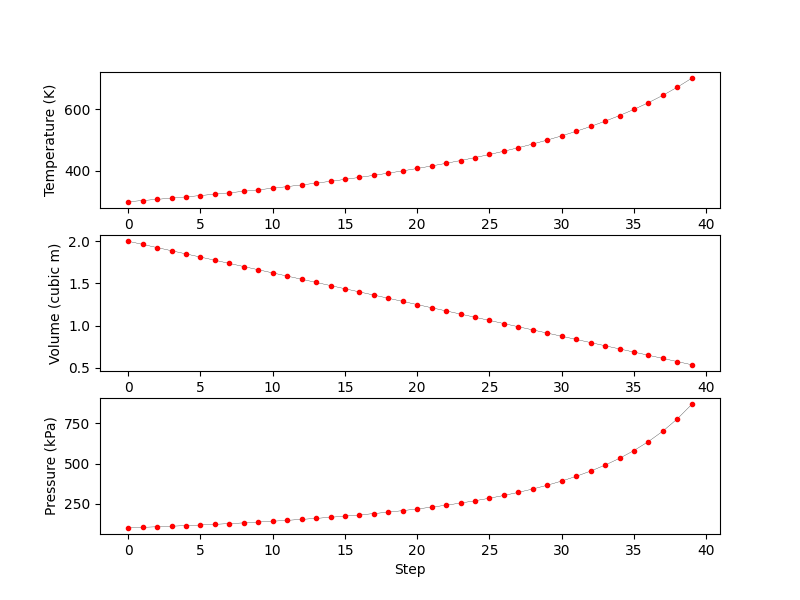
\includegraphics[width=\textwidth]{chunkplot1.png}

But, we will get better estimates if we break it up into 400 steps instead of 40.    Change the line that defines the number of steps:

\begin{Verbatim}
step_count = 400 # steps
\end{Verbatim}

Now the predicted temperature and pressure should be something like $753.603^\circ$  K and 1004.803 kPa.   (This is much closer to the correct result: :$755.953^\circ$ K and 1007.937 kPa.)

What if you break it into 400,000 steps?  Now the result should be really, really close to correct.  And the plot is quite accurate:

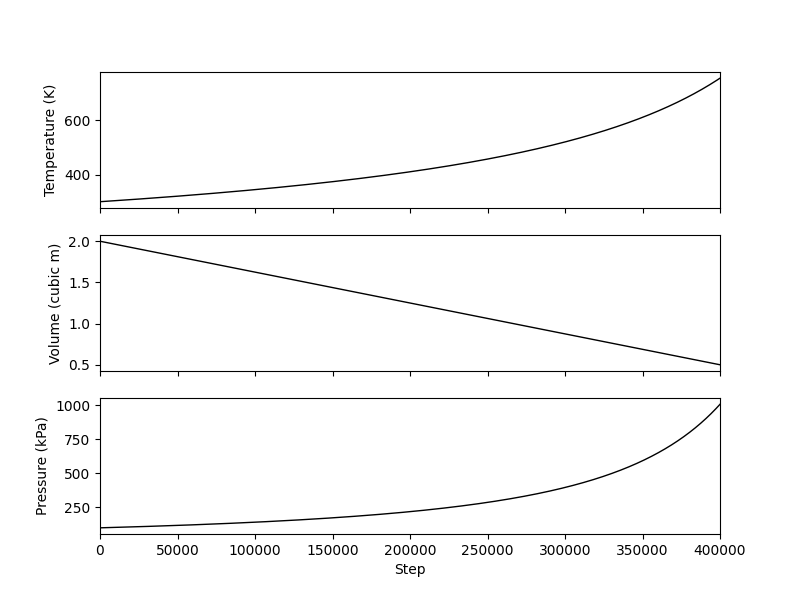
\includegraphics[width=\textwidth]{chunkplot2.png}

(You can comment out the lines that make the red dots on the graphs.  No
one wants to see 400,000 red dots.)

It is inefficient to have to do long simulations to guess the final temperature and pressure. Fortunately,  there are two handy rules you can use to skip this:

\begin{mdframed}[style=important, frametitle={Adiabatic Compression and Decompression}]

Let 

$$\gamma = \frac{C_{P,m}}{C_{V,m}}$$

In an adiabatic compression or decompression,  $P$ and $V$ change,  but

$$P \left(V^\gamma \right)$$

stays constant.

Also 

$$T \left(V^{\left( \gamma - 1 \right)} \right)$$

stays constant

\end{mdframed}

For a monoatomic gas:

$$\gamma = \frac{C_{P,m}}{C_{V,m}} = \frac{5}{3}$$

$$\gamma - 1 =  \frac{2}{3}$$

Before the compression: 

$$T \left(V^{\left( \gamma - 1 \right)} \right) = 300 \left( 2^{0.6667} \right) = 476.22$$

After the compression it has to be the same:

$$T \left(V^{\left( \gamma - 1 \right)} \right) = T \left( 0.5^{0.6667} \right) = 476.22$$

Thus 

$$T = 755.95^\circ \text{ Kelvin}$$

We can then use the ideal gas law to solve for the final pressure:

$$P = \frac{n R T}{V}  =  \frac{(80.18)(8.31446)(755.95)}{0.5} = 1007937 \text{ pascals}$$

That's hot!  As you let it cool back down to 300 degrees Kelvin,  how much heat would be released?  

$$E = C_{V,m} n \Delta T = (12.47)(80.2)(755.95 - 300) \approx  456 \text{ kJ}$$

\section{How an Air Conditioner Works}

Once again, imagine the accordion-like container filled with helium.  Let's say you walked it outside and compressed it from 2 cubic meters to 0.5 cubic meters in a vise.  The container would get to 755.95 degrees Kelvin.  You keep it compressed, in the vise  but let it cool down outside.  When it gets back to 300 degrees Kelvin,  you walk it back inside.

Now,  without letting any molecules in or out of the container,  you release the vise.  The gas is decompressed and gets very cold -- how cold?  Cold enough to accept about 456 kJ of kinetic energy from your house.  That is,  it would absorb heat from your house until the gas inside was the same temperature as your house.

Now you walk outside with your accordion and your vise and repeat:
\begin{enumerate}
\item Compress the gas outside.
\item Let the hot gas cool down outside.
\item Walk the room-temperature compressed gas inside.
\item Decompress the gas inside.
\item Let the cold gas warm up inside.
\end{enumerate}

You could keep your house cool on a hot day this way.  And this is not unlike how an air conditioner works.

There is a hose filled with refrigerant that does a loop:  
\begin{itemize}
\item Outside,  the refrigerant is compressed and allowed to cool to the outside temperature.  (Usually there is a big fan blowing on a coil of refrigerant to speed the process.)
Inside,  the refrigerant is decompressed and allowed to warm to the inside temperature.  (Usually there is a big fan blowing the air of the home past a coil of refrigerant to speed the process.)
\end{itemize}

In each pass of the loop,  the refrigerant absorbs some of the kinetic energy from inside the house, and releases it on the outside.

This same mechanism can be used to heat your house.  (Units that both heat and cool are known as \newterm{heat pumps}.)  
The heat pump does the process backwards:  The hot compressed refrigerant cools down inside.  The cold decompressed refrigerant warms up outside.


\graphicspath{{../../Chapters/phase_change/en_US}}
\chapter{Phases of Matter}

You have experienced $H_2O$ in three phases of matter:
\begin{itemize}
\item Ice is $H_2O$ in the solid phase.  At standard pressure,  when the temperature of $H_2O$ is below $0^\circ$ C,  it is a solid.  
\item Water is $H_2O$ in the liquid phase.  At standard pressure, when the temperature of $H_2O$ is between $0^\circ$ C and  $100^\circ$ C,  it is a liquid.
\item Water vapor (or steam) is the gas phase.  At standard pressure,  when the temperature of $H_2)$ is above $100^\circ$ C,  it is a gas.
\end{itemize}

Let's look at some of the properties of the three phases:

\begin{tabular}{p{5cm}|p{5cm}|p{5cm}}
Gas & Liquid & Solid \\
\hline
Assumes the volume and shape of its container & 
Assumes the shape, but not the volume, of its container &
Retains its shape and volume \\
\hline
Compressible & Not compressible & Not compressible \\
\end{tabular}

\section{Thinking Microscopically About Phase}

As mentioned in an early chapter,  there are intermolecular forces that attract molecules to each
other.   A pair of molecules will have very strong intermolecular forces or very weak intermolecular forces
depending on what atoms they are made of.

For example,  two helium molecules are very weakly attracted to each other due to weak intermolecular forces.   Two molecules of $NaCl$ (table salt) will experience very strong intermolecular attraction.

In a gas,  the molecules have lots of room to roam and lots of kinetic energy: The intermolecular attraction has very little effect.

In a liquid,  the molecules are sticking close together,  but are still moving around,  sort of like bees in a hive.

In a solid, the molecules are not changing their configuration, and the kinetic energy they have is just expressed as vibrations within that configuration.   You can imagine them like eggs in a carton just vibrating.

As you would expect, molecules with strong intermolecular attraction require more kinetic energy to change phases.  For example,   helium is a liquid below $-269\circ$ C.  $NaCl$, on the other hand, is a liquid between $801^\circ$ and $1,413^\circ$ C.  

The temperatures I just gave you are at standard pressure (100 kPa or 1 atm).  Pressure also has a role in phase change:  In low pressure environments,  it is much easier for the molecules to make the jump to being a gas.

For example,  if you climb a mountain until the atmospheric pressure is 70 kPa,  your water will boil at about $90^\circ$ C.  

If you rise in a balloon until the atmospheric pressure is 500 Pa,  if your water is colder than $-2^\circ$ C,  it will be ice.  If it is warmer it will vaporize.    There is no liquid water at 500 Pa!

For any molecule,  we could observe its phase at a wide range of temperatures and pressures.  This would let us create a phase diagram.  Here is the phase diagram for $H_2O$:

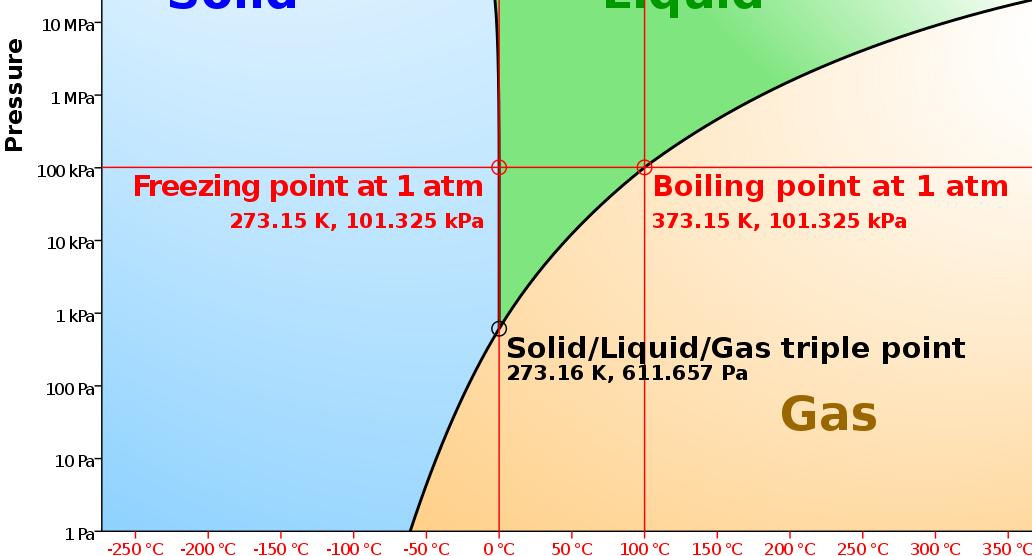
\includegraphics[width=\textwidth]{waterphase_edit.png}

(FIXME: This diagram needs to be recreated prettier.)

\section{Phase Changes and Energy}

The molar heat capacity of ice is about 37.7 J/mol-K.  That is it takes about 37.7 Joules of energy to raise the temperature of one mole of ice by one degree kelvin.

The molar heat capacity of liquid water is about 75.4 J/mol-K.  For water vapor, it is about 36.6 J/mol-K.

Imagine you have mole of ice at $173^\circ$ K  and you are going gradually add kinetic energy into it until you have steam at $473^\circ$ K.  You might guess (wrongly) that the temperature vs. energy applied would look like this:

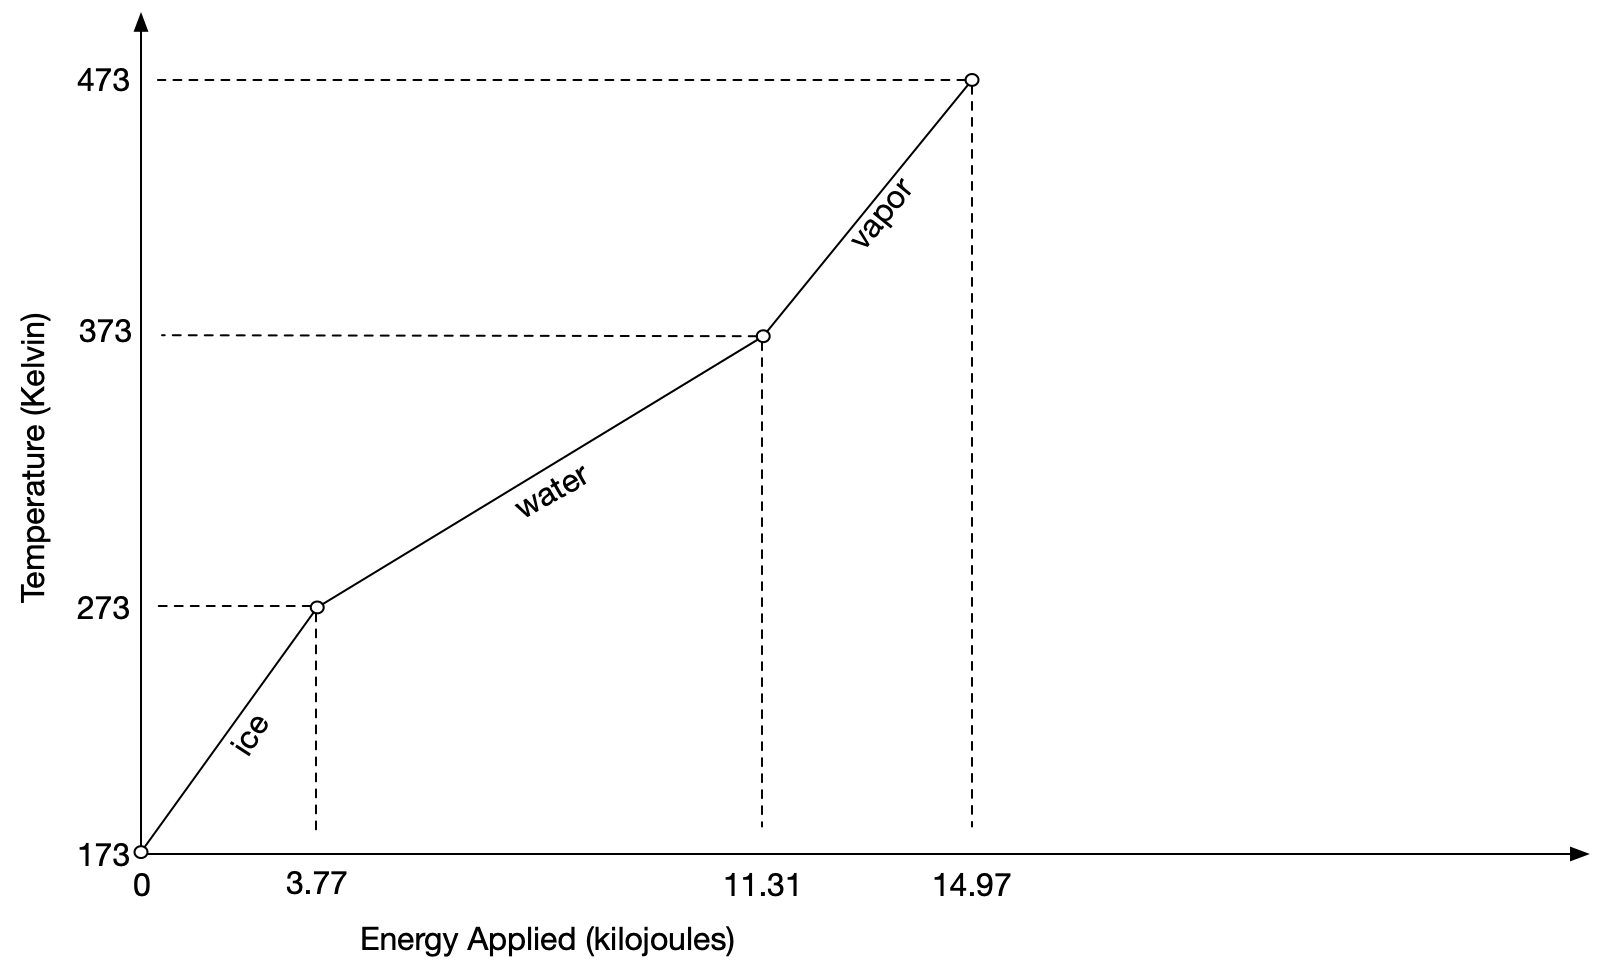
\includegraphics[width=0.8\linewidth]{energynaive.png}

However,  once molecules are nestled into their solid state (like eggs in cartons),  it take extra energy to make them move like a liquid.  How much more energy?  For water,  it is 6.01 Joules per mole.  This is known as \newterm{the latent heat of melting}

Similarly,  the transition from liquid to gas takes energy.  At standard pressure,  converting a mole of liquid water to vapor requires 40. 7 Joules per mole.  This is known as \newterm{the latent heat of vaporization}. So the graph would actually look like this:

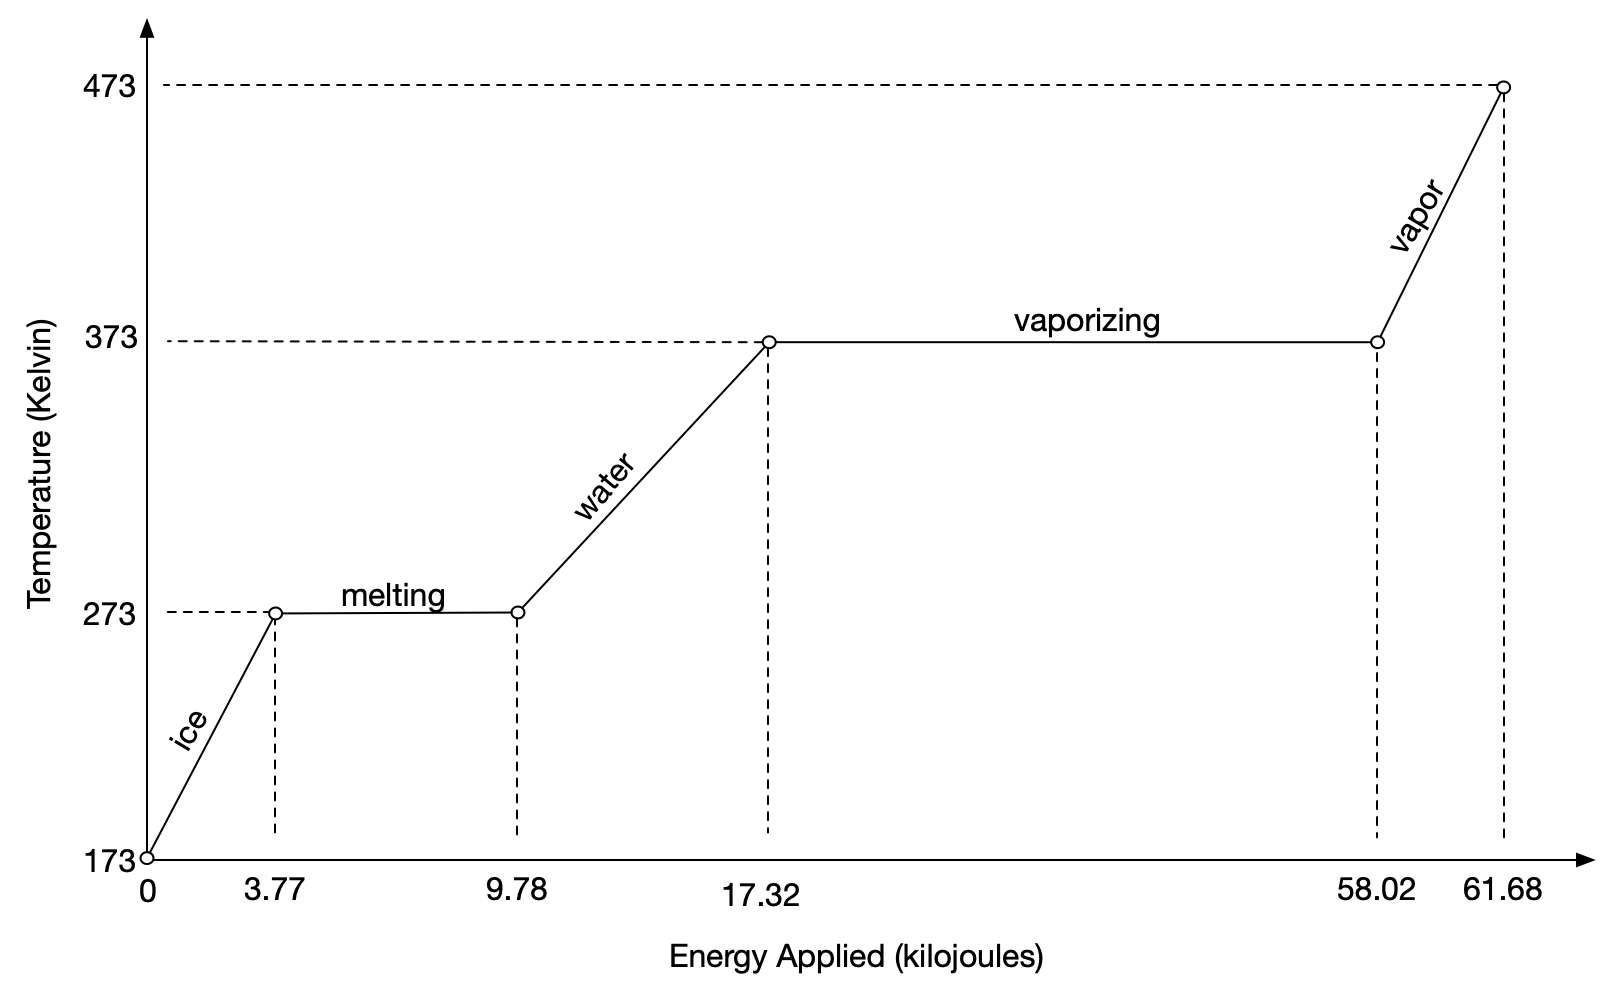
\includegraphics[width=0.8\linewidth]{energysoph.png}

Note that just as melting and vaporizing require energy.   Going the other way (freezing and condensing, respectively) give off energy.    Thus, we can store energy using the phase change.

\section{How a Rice Cooker Works}

As you might imagine,  a rice cooker is a bowl with a lid and an electric heating element.  You put rice and water into the bowl and turn on the heating element.   The heating element pushes kinetic energy into the water, which gets warmer and eventually starts to boil.

How does the rice cooker know when to turn off (or at least down to a low-heat "keep warm" mode) before the rice starts to burn?

As long  as there is a little liquid water in the bottom of the bowl, the rice won't burn, so the question really is "How does it know when there is no more liquid water in the bottom of the bowl?"

There is a mechanism (and there have been a few different versions of this mechanism)  that monitors the temperature of the surface of the bowl.  As long as there is liquid water in the bowl,  it \emph{cannot} go above $100^\circ$ C!  When all the water has been absorbed by the rice or turned to steam,  the temperature rises above $100^\circ$ C, and the mechanism cuts off the heat.

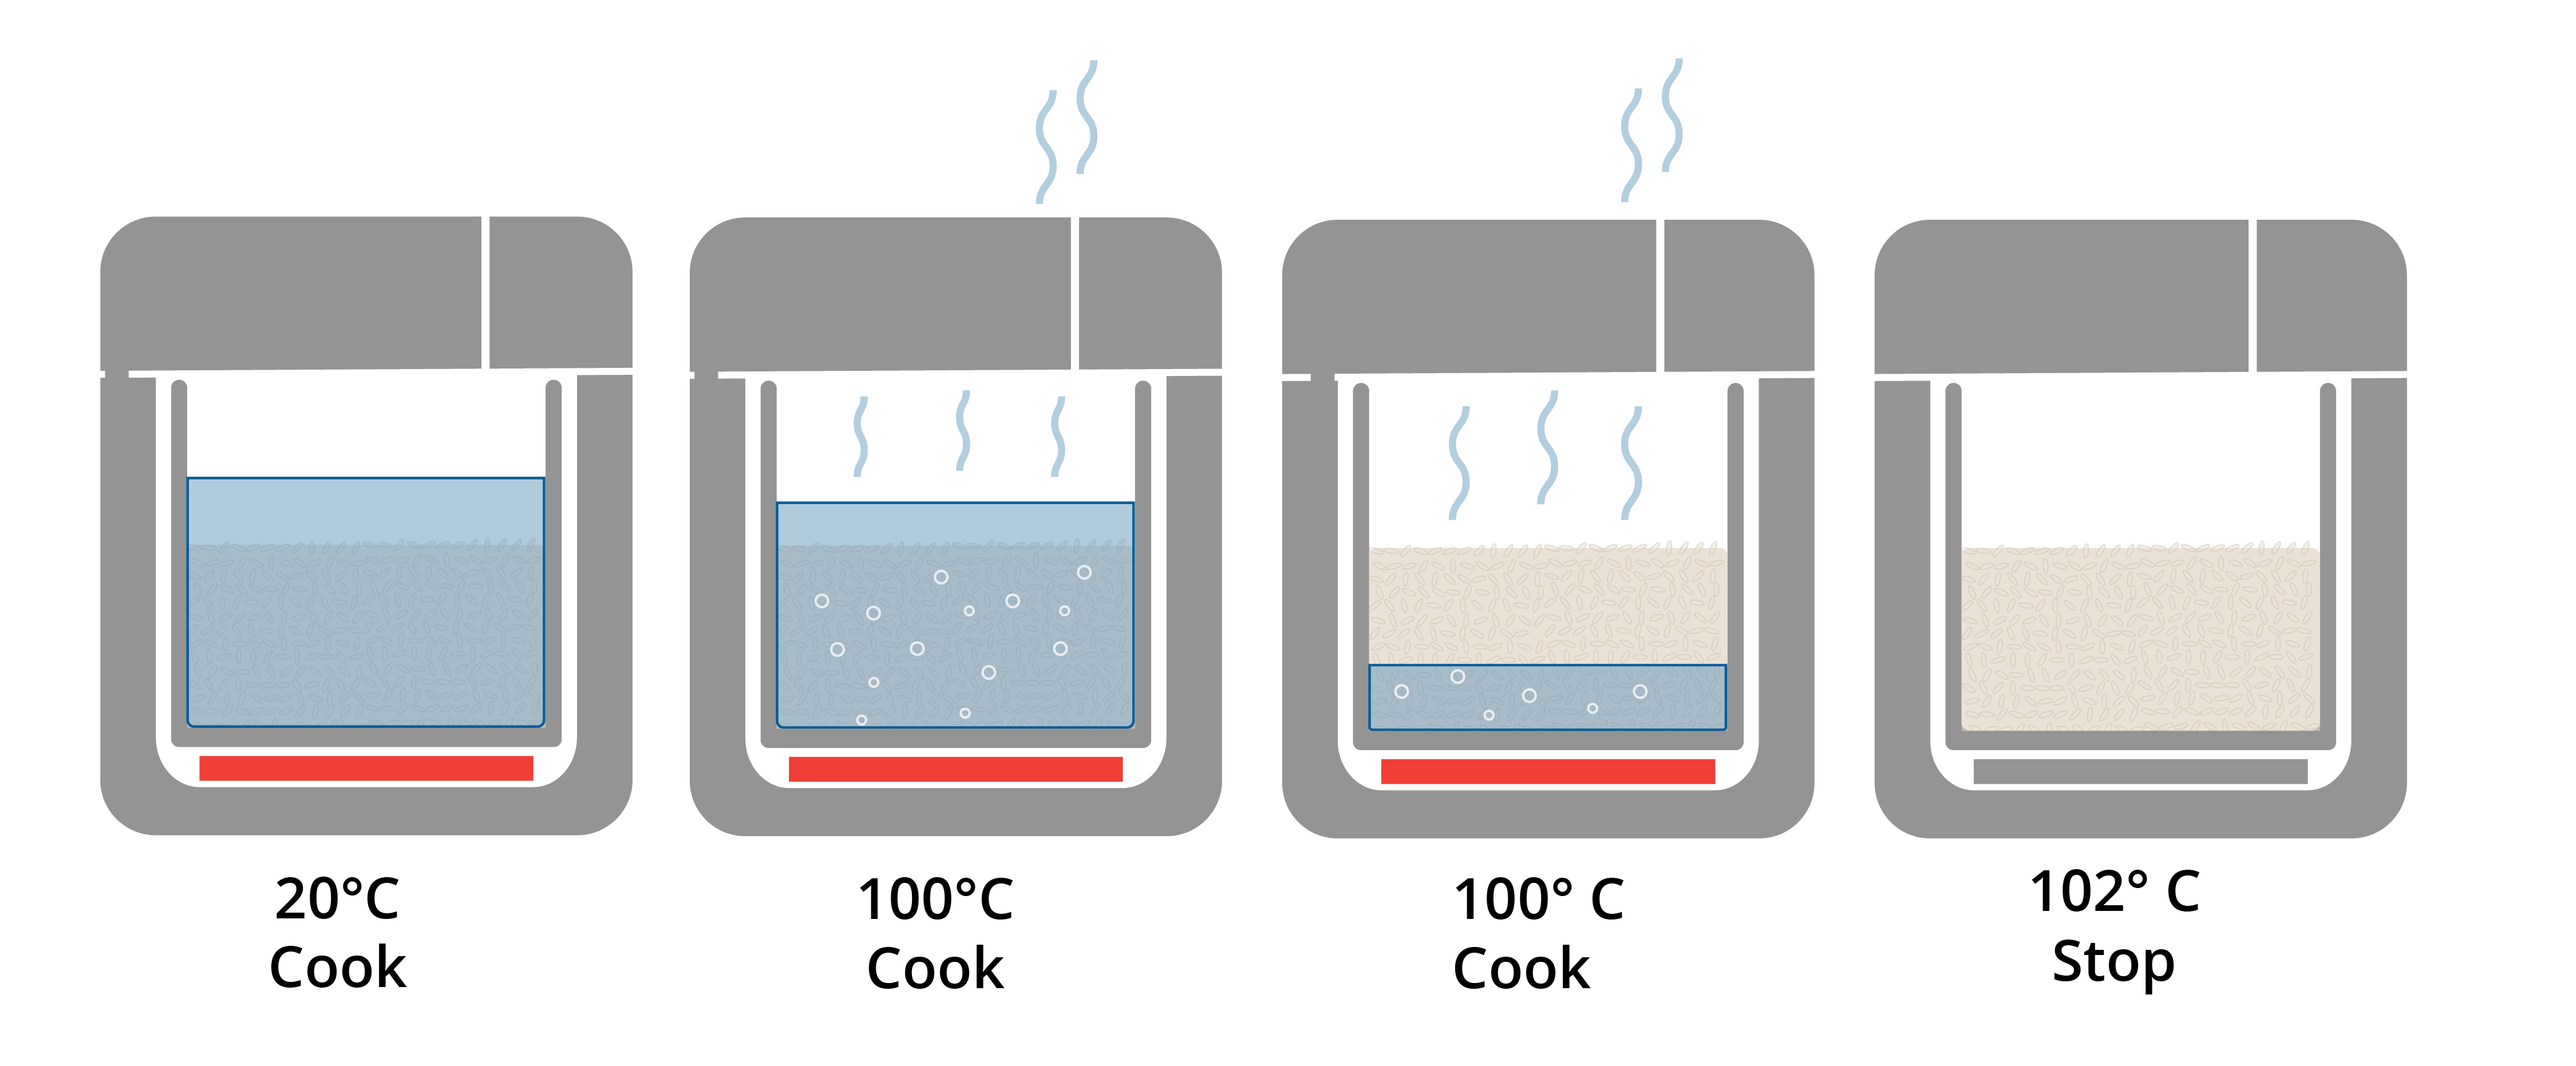
\includegraphics[width=0.9\linewidth]{riceCookerPhase.png}

\begin{Exercise}[title=Using Water For Thermal Energy Storage, label=waterthermal]
Tom is building a passive solar house:  the front of his house is a greenhouse.  He also likes to 
eat dinner in the greenhouse.  He will have barrels (painted black) that hold 159 liters of water.  His plan is to let the sun heat the barrels to $33^\circ$ C by the time the sun goes down.  (Any warmer and it would be unpleasant to eat dinner near them.)

At night, he will circulate air past the barrels and through his house.  He is OK with the house and the barrels dropping to $17^\circ$ C.

Looking at the insulation on his house and the expected nighttime temperatures,  Tom estimates that he needs to store 300,000 KJ of energy in the barrels.

A mole of water is about 0.018 liters.

The molar heat capacity of water is about 75.38 J/mole-K.

How many barrels of water does Tom need to install in his greenhouse?

\end{Exercise}
\begin{Answer}[ref=waterthermal] 

When one mole of water goes from $33^\circ$ to $17^\circ$,  it will give off $(75.38)(33-17) = 1,206$ Joules or $1.206$ kJ. 

Tom needs 300,000 kJ,  so he needs $300,000/1.206 =   248,739.72$ moles of water.

How many liters is that?  $248,739.72 * 0.018 = 4,477.31$ liters.

How many barrels is that? $4,477.31 / 159 = 28.16$ barrels.  He will need 29 barrels.
  
\end{Answer}


\begin{Exercise}[title=Using Mirabilite For Thermal Energy Storage, label=mirabilite]

Water barrels are going to take up too much of Tom's greenhouse!

There is a substance known as mirabilite, or Glauber's salt,  or sodium sulfate decahydrate.  It is relatively cheap to produce, and it has a melting point of $32.4^\circ$ C.

The molar heat capacity of mirabilite is 550 J/mole-K.

The latent heat of melting mirabilite is 80 KJ per mole.

Mirabilite comes in a powder form.  Assume that a mole of mirabilite occupies about 0.22 liters.

If Tom fills his barrels with mirabilite,  how many barrels will he need?

\end{Exercise}
\begin{Answer}[ref=mirabilite] 

When one mole of mirabilite goes from $33^\circ$ to $17^\circ$,  it will give off $(550)(33-17) + 80,000 = 88,800$ Joules or $88.8$ kJ. 

Tom needs 300,000 kJ,  so he needs $300,000/88.8 =   3,378$ moles of mirabilite.

How many liters is that?  $3,378 * 0.22 = 743.24$ liters.

How many barrels is that? $743.24 / 159 = 4.67$.  He will need 5 barrels.
  
\end{Answer}



%%%%%%%%%%%%%%%%%%%%%%%%%%%%%%%%%
%% Bookfooter.tex by Aaron Hillegass
%% Nov 8, 2020

\appendix

\chapter{Answers to Exercises}
\shipoutAnswer

\bibliography{references}

\printindex

\end{document}